\chapter{Model Personalisation}
\label{chp:personalisation}

The previous chapter investigated classification accuracy for a subject agnostic \acrshort{lstm} based \acrshort{lmr} model. The outcome of this was that accuracies of greater than 80\% were not possible for unseen novel subjects. Instead a bespoke/personalised \acrshort{lmr} model is necessary to achieve higher performance. Within this chapter methods for achieving this will be explored.

% Relevant background on the topic - For a paper describing original research, you’ll instead provide an overview of the most relevant research that has already been conducted. This is a sort of miniature literature review—a sketch of the current state of research into your topic, boiled down to a few sentences.
The collection of labels from every individual is burdensome therefore any system that can be used to reduce the labelled data requirements is advantageous. This can be achieved through the use of a larger global source training set pooled from many individuals in the assumption they will hold information relevant to the target individual.\cite{Fallahzadeh2017, Schneider2021} 

Following the convention of transfer learning the personalisation subjects will be refereed to as the target. All other subjects which form prior knowledge will be referred to as source.

% Research question
% Present your research question clearly and directly, with a minimum of discussion at this point. The rest of the paper will be taken up with discussing and investigating this question; here you just need to express it.
Within this chapter we will investigate whether a large population of source data can be effectively used to improve the performance of a target individual's \acrshort{lstm} based \acrshort{lmr} classifier.

% Sometimes an overview of the chapter
The Chapter is presented as follows. Firstly, in Section \ref{sec:personalisation-related-works}, related literature is presented. This is followed by the methods and materials used in the study in Section \ref{sec:personalistaion-methods}. The results of a baseline model trained from only target data are presented in Section \ref{sec:personalisation-baseline-model-results}, followed by the results and analysis for penalisation techniques in Section \ref{sec:model-personalisation-results}.  Finally discussion and conclusions are presented in Sections \ref{sec:personalisation-discussion} and \ref{sec:personalisation-conclusions} respectively.


%------------------------------------------
\section{Related Works}
\label{sec:personalisation-related-works}
% Establish your research problem
% In an empirical research paper, try to lead into the problem on the basis of your discussion of the literature. Think in terms of these questions:
% What research gap is your work intended to fill?
% What limitations in previous work does it address?
% What contribution to knowledge does it make?
% What are common ways personalistaion is achieved

\acrshort{ml} classifiers are constructed with the assumption that the data distribution between the general source data domain and the new novels subject target domain are equal\cite{Farahani2020}. In reality this is never the case, as such a form of personalisation or domain adaption is required to allow for accurate classification in the target domain.

%What are the issues that we've identified and how are they commonly solved in literature.
Personalising of \acrshort{ml} models is a common issue and has been addressed in many different ways across different disciplines\cite{Mairittha2021, Tomanek2021}. Schneider et al divide personalising methods into two groups, shaping and data grouping\cite{Schneider2021}. The survey of literature will be divided into these two groups. Both of these techniques take advantage of data from other subjects to reduce labelled data requirements for the target subject\cite{Shor2020}.

% Shaping/transfer learning Early shaping train with target then source, late train with source then target, sample weighting - weighting the training data -- seems like data grouping.
In shaping the behaviour of a network is shaped toward a individual. This is commonly done in two ways early and late. In early shaping an target data is first used to train a model followed by source data. The opposite is done in late shaping. The last method is refereed to as transfer learning.\cite{Schneider2021}

Transfer learning is the ability to extend what has been learnt in one context to another nonidentical but similar context\cite{Fallahzadeh2017}. Transfer learning is appealing, since it is potentially faster as it is not necessary to train the model from scratch for each target individual.

By updated a trained model using data from a different distribution, an the knowledge from an existing model can be transferred. Where the model remains the same transfer learning is generally achieved in two phases, first a generic global model is trained from source data. Then it is personalised for the individual by additional training using only the targets data. The influence of the individual is controllable by both the number of iterations and number of layers trained.\cite{Schneider2021, Mireshghallah2021}

% EXAMPLES OF SHAPING/TRANSFER LEARNING IN HAR
Yoon et al
% Retrain general model
Personalised language modelling using RNN - no examples of transfer learning for HAR in RNN. "It trains a base model with a large dataset and copies its first n-many layers to the first n-many layers of a target model. Then the target model is fine-tuned with relatively small target data. Several learning schemes such as freezing a certain layer or adding a surplus layer are pro- posed for achieving the result."\cite{Yoon2017}

Wang et al does x
deep transfer learning - knowledge transfer between different data sets with sensors in different places\cite{Wang2018a} "when there are several source domains available, it is difficult to select the right source domains for transfer. The right source domain means that it has the most similar properties with the target domain, thus their similarity is higher, which can facilitate transfer learning" "Unsupervised Source Selection algorithm for Activity Recognition (USSAR). USSAR is able to select the most similar K source domains from a list of available domains. Af- ter this, we propose an effective Transfer Neural Network to perform knowledge transfer for Activity Recognition"

Fu et al
% Domain adaptation - Create mapping between similar subjects
Joint probability domain adaptation and improved pseudo labels\cite{Fu2021}. Manually selected features. Domain adaptation through selection of a mapping function between source and target features. 93.3\% accuracy of target domain


%-----------------------------
% Data grouping
``With data grouping, we aim at enlarging the data of an individual DI by adding similar data. Then, instead of shaping with the small dataset DI, we utilize the enlarged dataset of the individual I. While each individual differs from each other, it can be expected that either entire datasets of individuals are similar or that for a sample there exist similar samples (originating potentially from different individuals).''\cite{Schneider2021}

%EXAMPLES OF DATA GROUPING IN HAR
Ferrari et al
% Training from similar users
Similarity based personalisation strategies. Comparison of physical characteristics of different subjects\cite{Ferrari2020}. Adaboost classifier. Train using data from a general population, with and without some of the target subject's data. Similarity between different subjects is used to weight the influence of a subjects data.

Nguyen et al "Each subject might exhibit user-specific signal patterns, yet a group of users may perform activities in simi- lar manners and share analogous patterns. Leveraging this intuition, we explore Frechet Inception Distance (FID) as a distribution matching- based metric to measure the similarity between users. From that, we propose the nearest-FID-neighbors and the FID-graph clustering tech- niques to develop user-specific models that are trained with data from the community the testing user likely belongs to." \cite{Nguyen2021}


%-----------------------------
% Combination - retrain general model based on similar users
Cruciani et al presents work on personalising an activity recognition model built from the subset of a general population. The subset of subjects was selected by comparing the similarity of manually selected features for the target subject and general training population. Those with the closest matching gait are used to generate the base model. Further training is then performed on this model using a small amount of the target subject data. This approach achieved a ~5\% improvement in performance when compared to selecting a subset at random\cite{Cruciani2020}. The experiment was performed on the \acrshort{adl} Extrasensory dataset published by Vaizman et al\cite{Vaizman2017}.


Research gaps
- Transfer learning in HAR has only used manually selected features - not learnt (deep) features
- Limited exploration of transfer learning for RNN in HAR


%------------------------------------------
\section{Methods and Materials}
\label{sec:personalistaion-methods}
Introduction to section

% Data collection
Extended the data set previously captured for a select subset of participants. The same methods as presented in Section \ref{sec:methods-data-collection} were used to collect this additional data.

Larger quantities of data collected for 3 subjects least 7-mins cumulative time of each activity class. 

%------------------
% Data augmentation (Combining left and right ankle data)
Mixed Left and Right ankle data - justification for doing this.

Figure \ref{fig:ch6_target_subject_gyro_trends} shows the mean signals from the shank mounted gyroscope in the saggital plane for each of the Target subjects. Data from the left ankle has been transformed in order that both ankles appear in the same axis.

Data is not normalised

Only stair descent for subject 03 shows meaningful differences between left and right ankles. Therefore it is acceptable to use data from both ankles.

\begin{figure}[p]
    \begin{tabular}{lccc}
        & \textbf{Subject 01} & \textbf{Subject 03} & \textbf{Subject 09} \vspace{0.2cm}\\

        \rotatebox{90}{\enspace\qquad \textbf{Walking}} &
        \begin{subfigure}[b]{0.275\textwidth}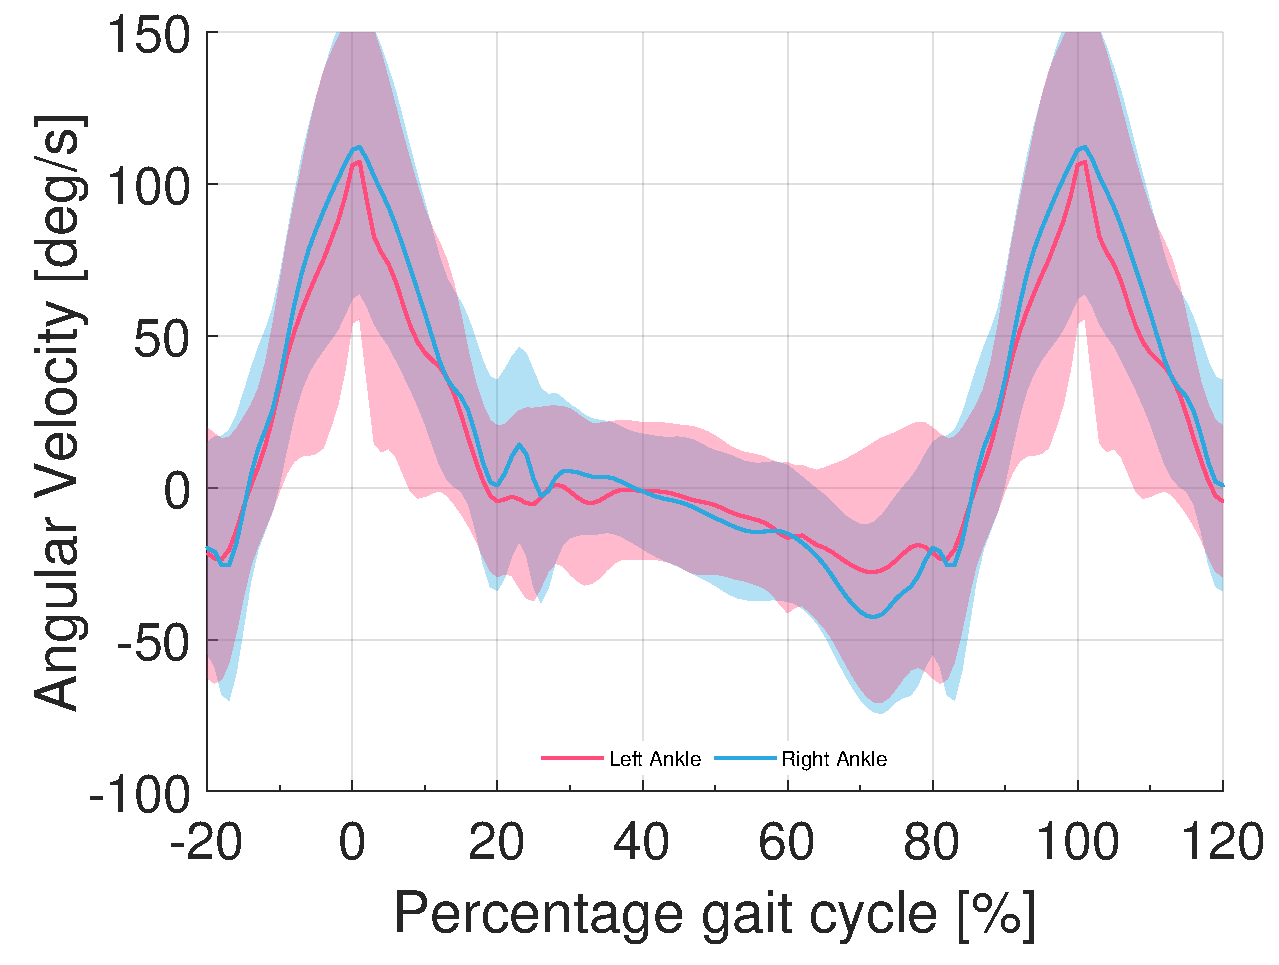
\includegraphics[width=\linewidth]{content/5-Personalisation/Gyro_Trends_For_Targets/ch5_gait_trends_subject_01_activity_walking.pdf}\end{subfigure} & \begin{subfigure}[b]{0.275\textwidth}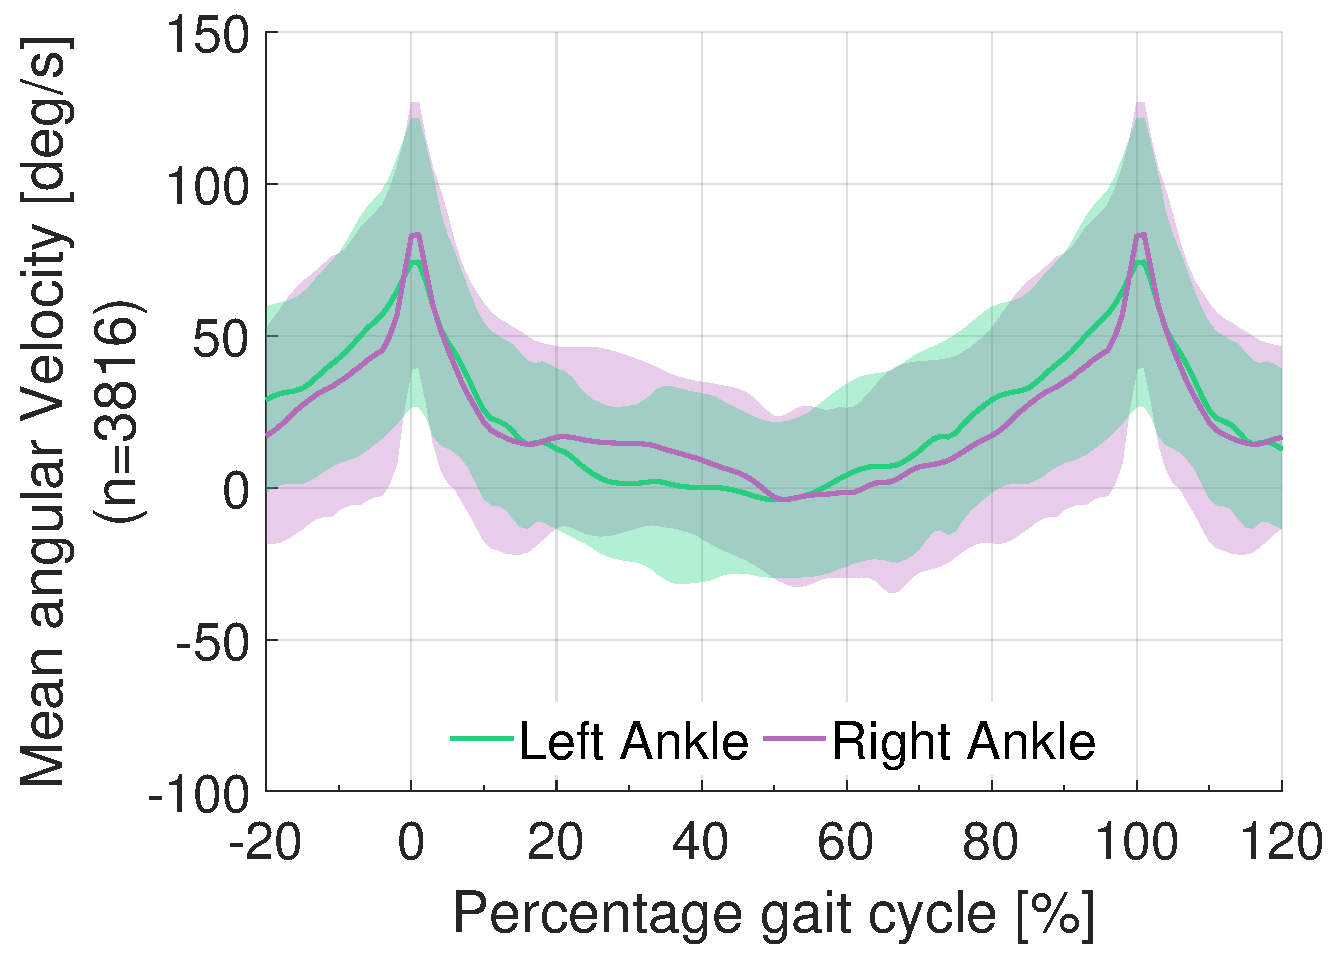
\includegraphics[width=\linewidth]{content/5-Personalisation/Gyro_Trends_For_Targets/ch5_gait_trends_subject_03_activity_walking.pdf}\end{subfigure} &
        \begin{subfigure}[b]{0.275\textwidth}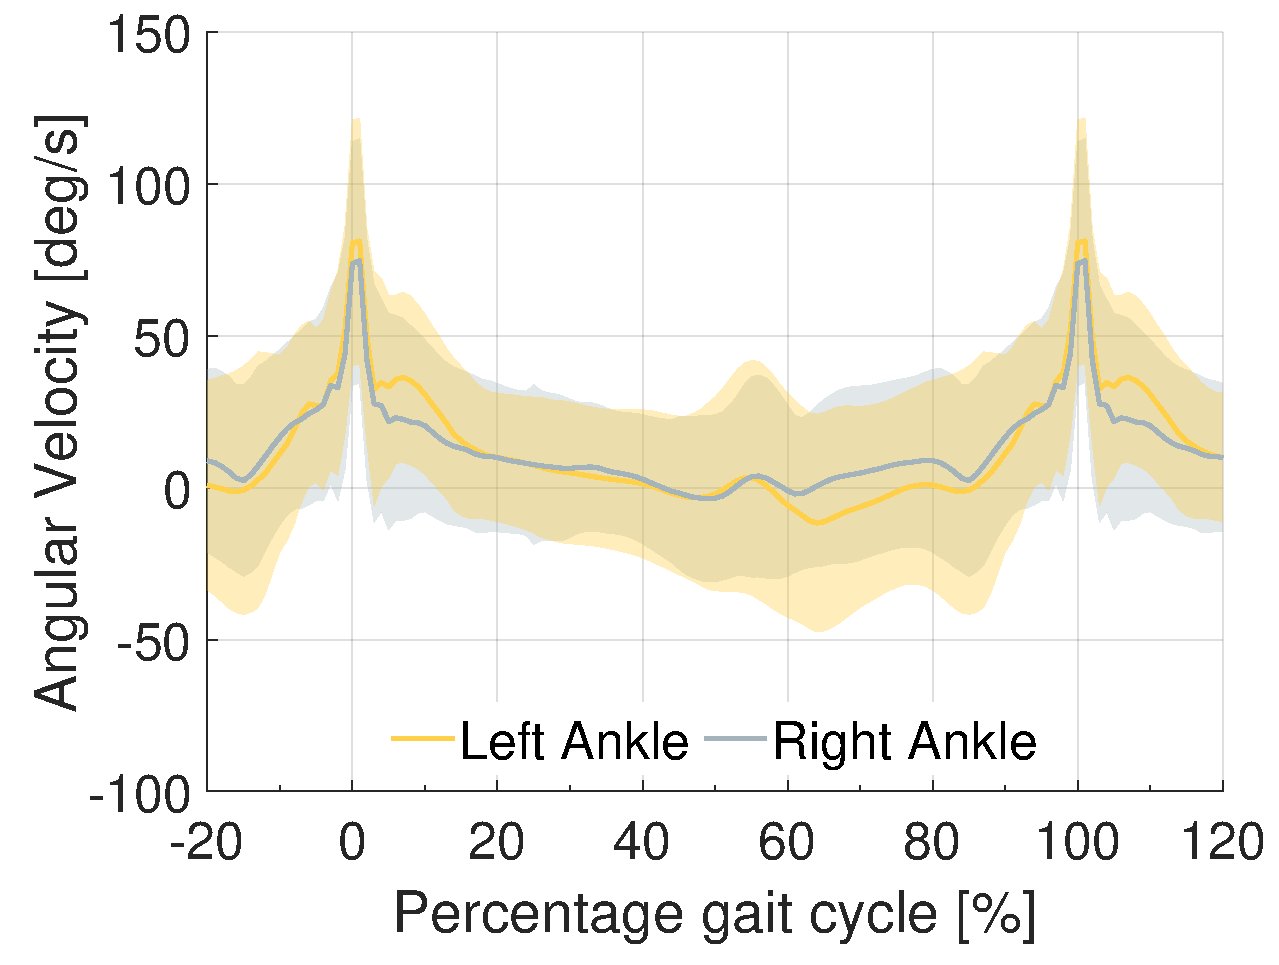
\includegraphics[width=\linewidth]{content/5-Personalisation/Gyro_Trends_For_Targets/ch5_gait_trends_subject_09_activity_walking.pdf}\end{subfigure} \\
        
        \rotatebox{90}{~\quad \textbf{\glsentrylong{ra}}} & 
        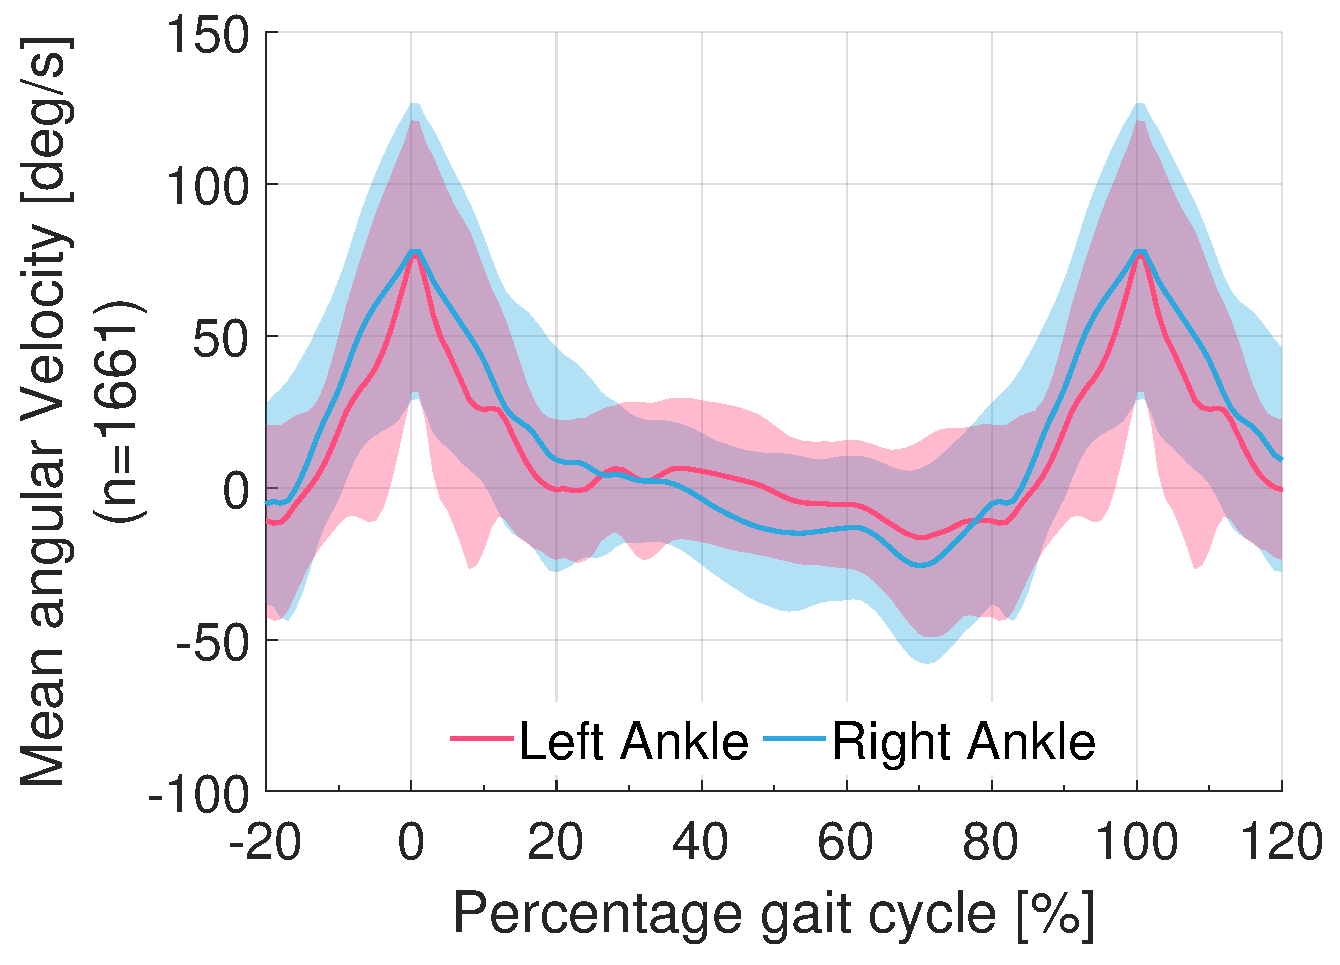
\includegraphics[width=0.275\linewidth]{content/5-Personalisation/Gyro_Trends_For_Targets/ch5_gait_trends_subject_01_activity_ramp_up.pdf} & 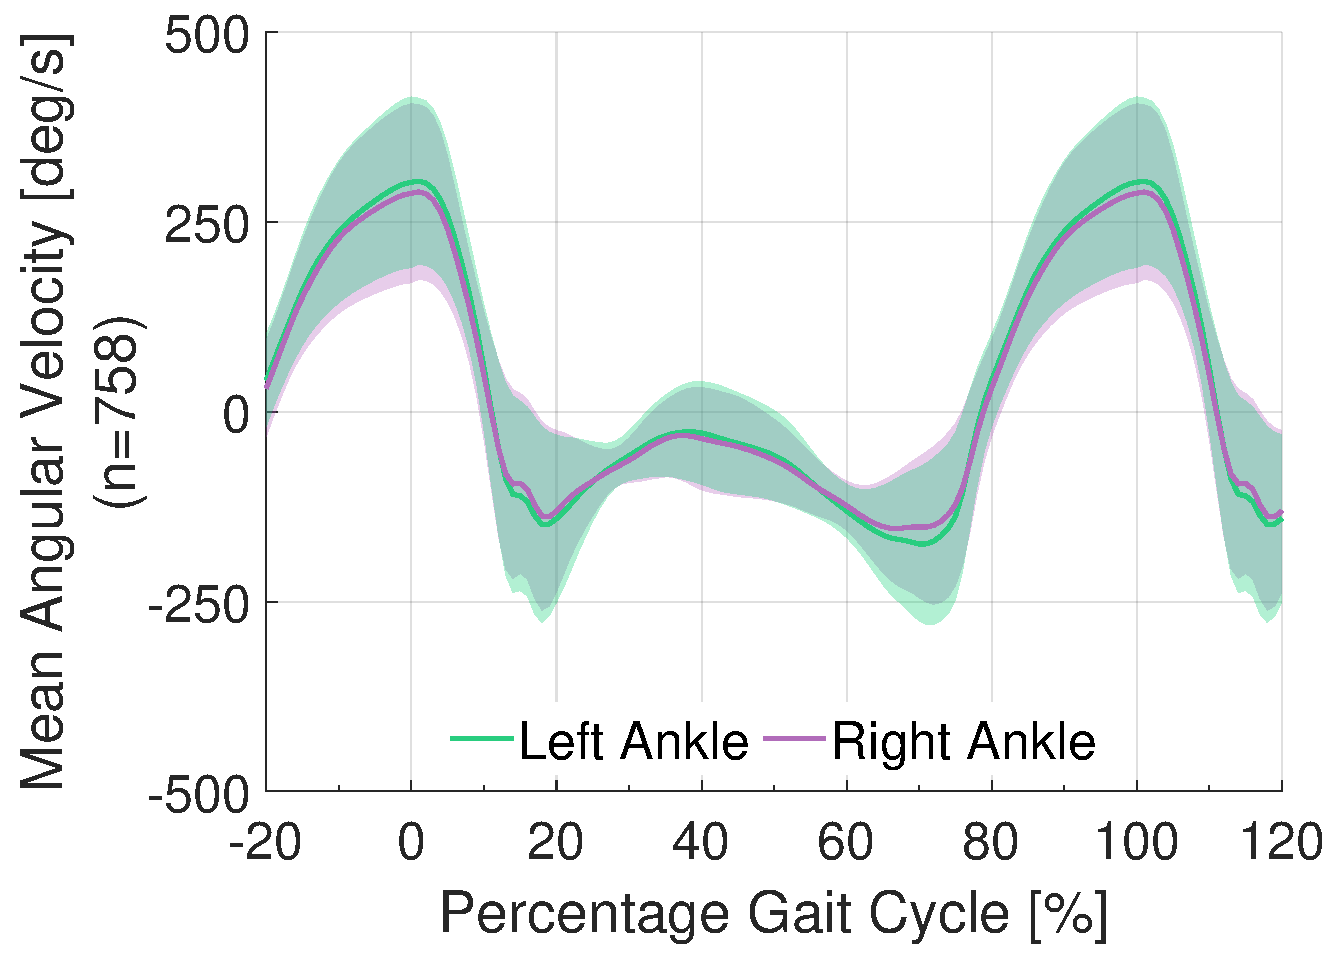
\includegraphics[width=0.275\linewidth]{content/5-Personalisation/Gyro_Trends_For_Targets/ch5_gait_trends_subject_03_activity_ramp_up.pdf} &
        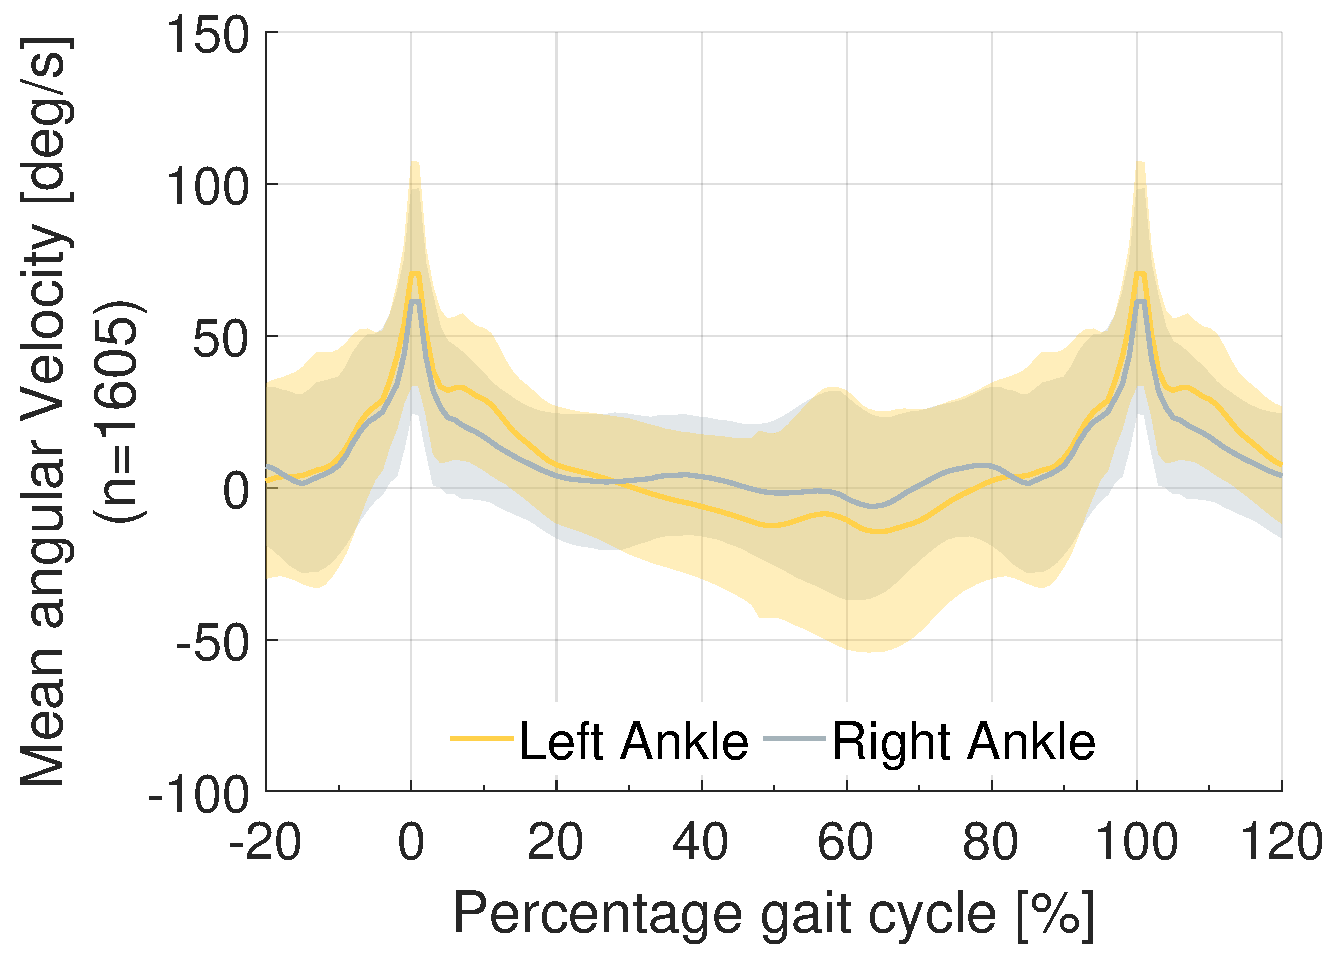
\includegraphics[width=0.275\linewidth]{content/5-Personalisation/Gyro_Trends_For_Targets/ch5_gait_trends_subject_09_activity_ramp_up.pdf} \\
        
        \rotatebox{90}{\quad \textbf{\glsentrylong{rd}}} & 
        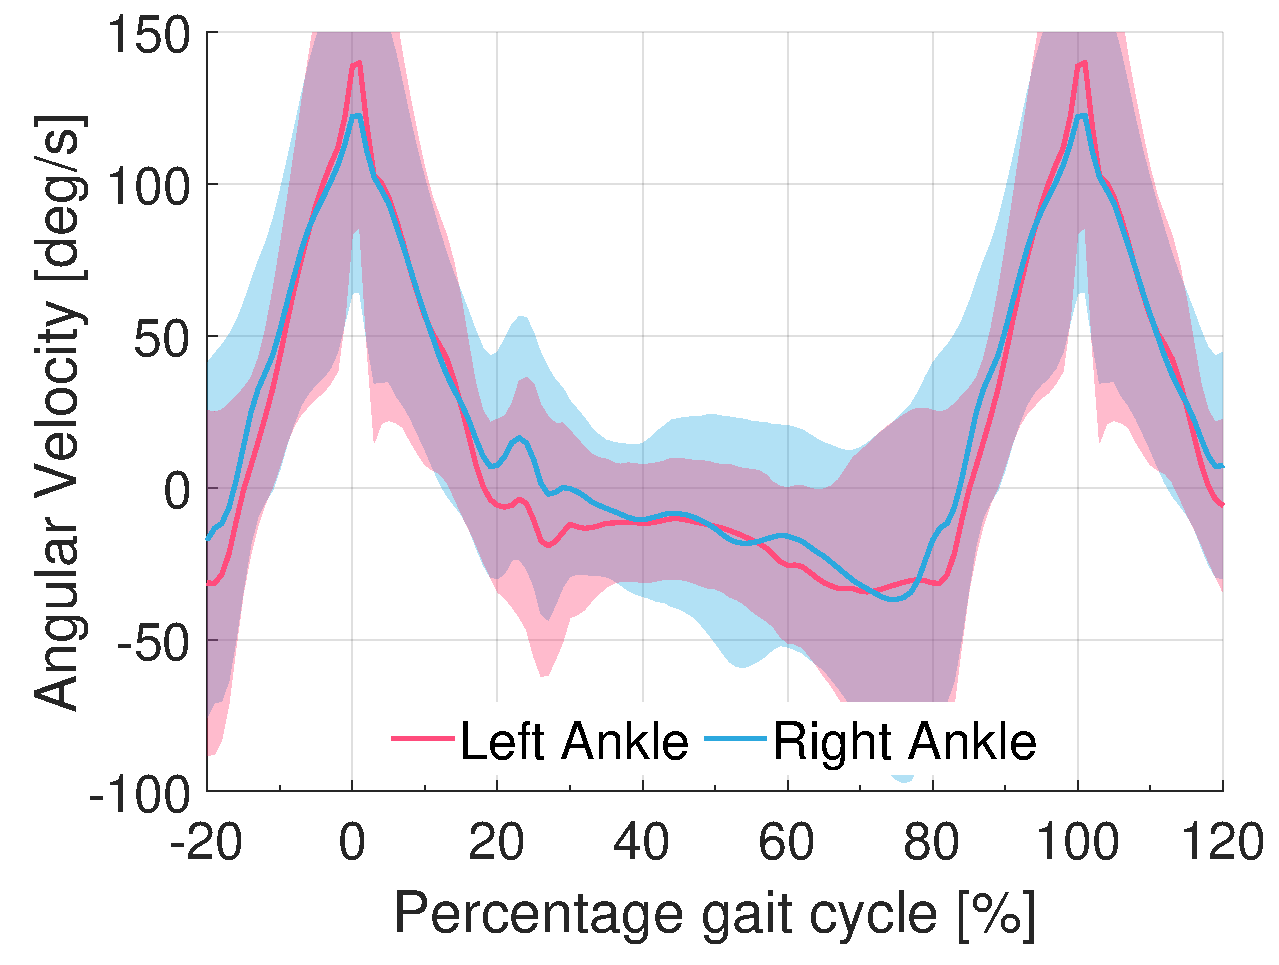
\includegraphics[width=0.275\linewidth]{content/5-Personalisation/Gyro_Trends_For_Targets/ch5_gait_trends_subject_01_activity_ramp_down.pdf} & 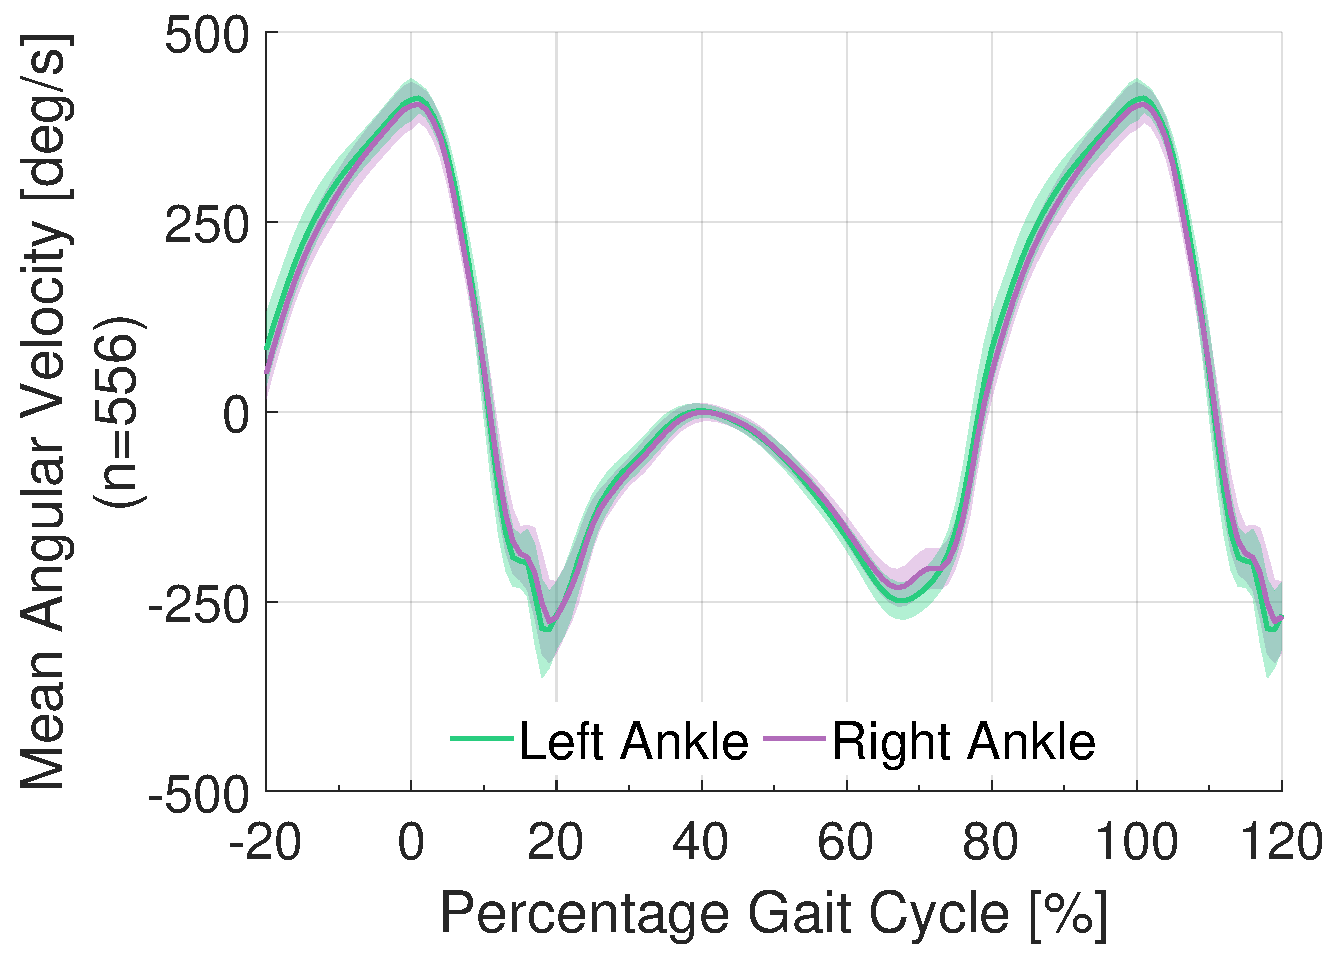
\includegraphics[width=0.275\linewidth]{content/5-Personalisation/Gyro_Trends_For_Targets/ch5_gait_trends_subject_03_activity_ramp_down.pdf} &
        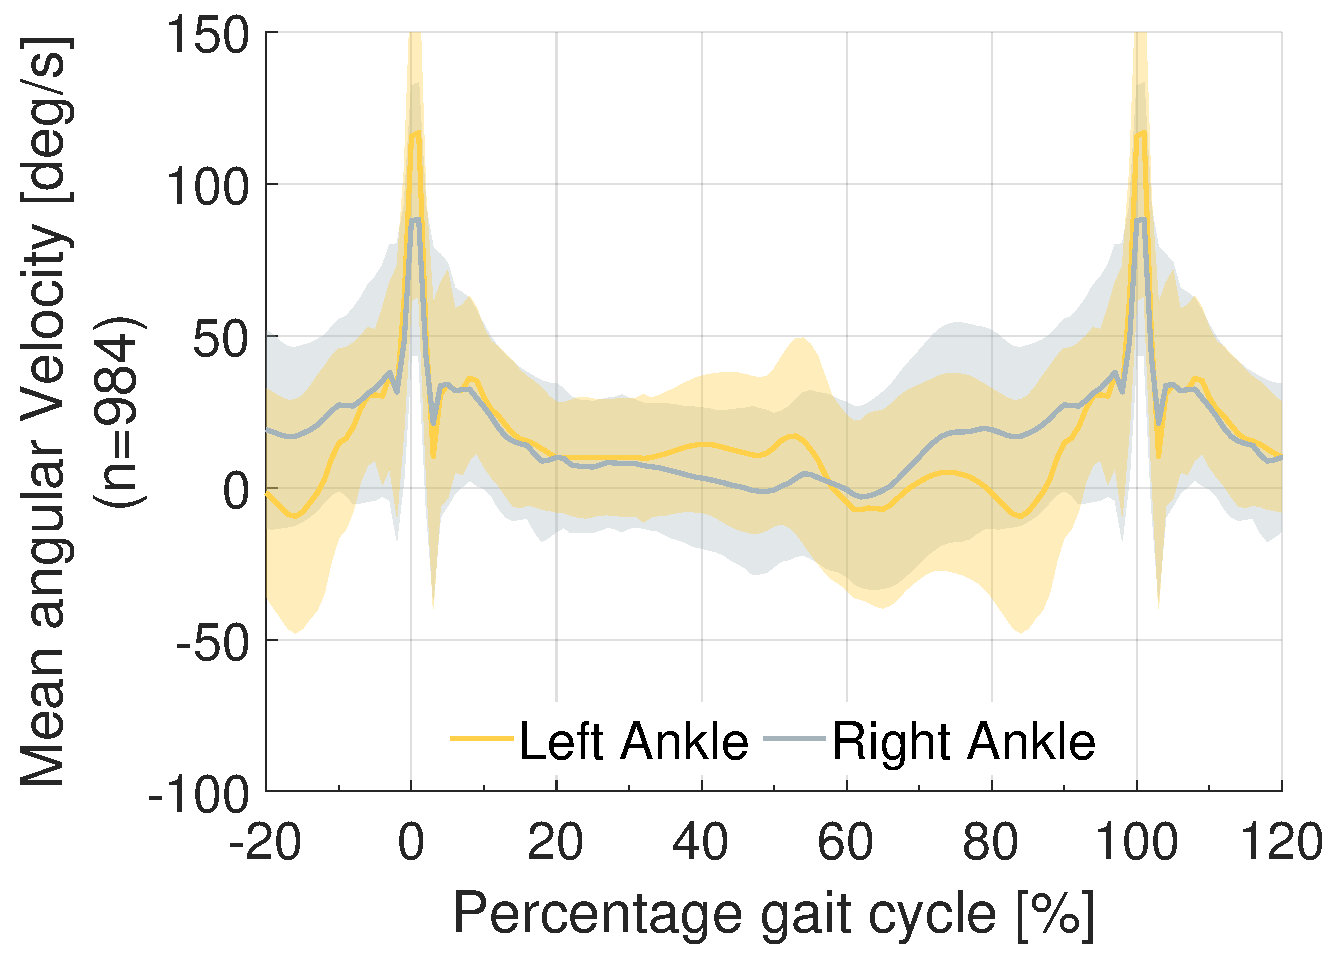
\includegraphics[width=0.275\linewidth]{content/5-Personalisation/Gyro_Trends_For_Targets/ch5_gait_trends_subject_09_activity_ramp_down.pdf} \\
        
        \rotatebox{90}{~\quad \textbf{\glsentrylong{sa}}} & 
        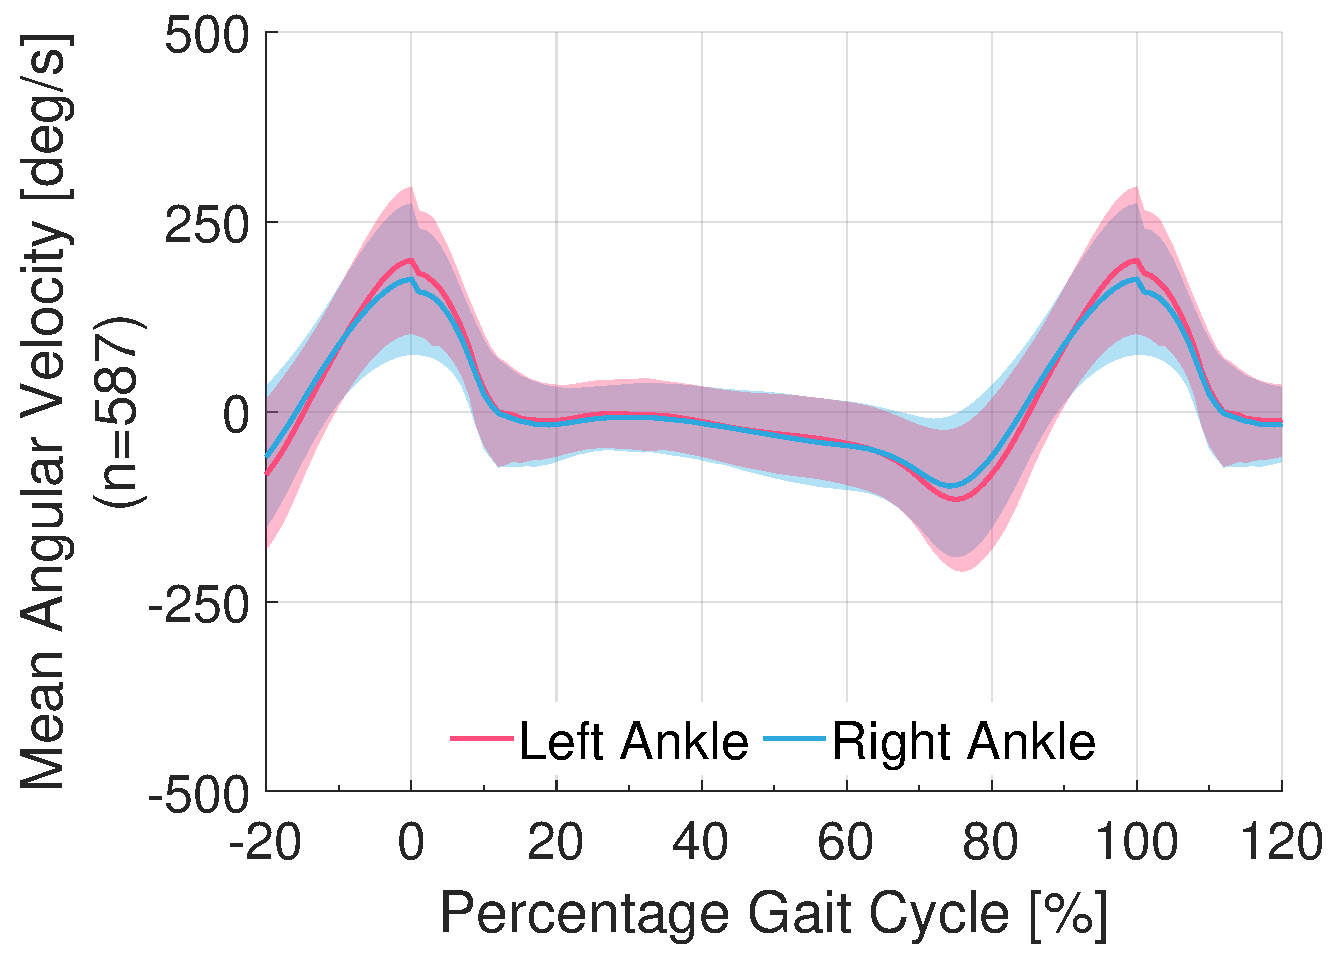
\includegraphics[width=0.275\linewidth]{content/5-Personalisation/Gyro_Trends_For_Targets/ch5_gait_trends_subject_01_activity_stair_up.pdf} & 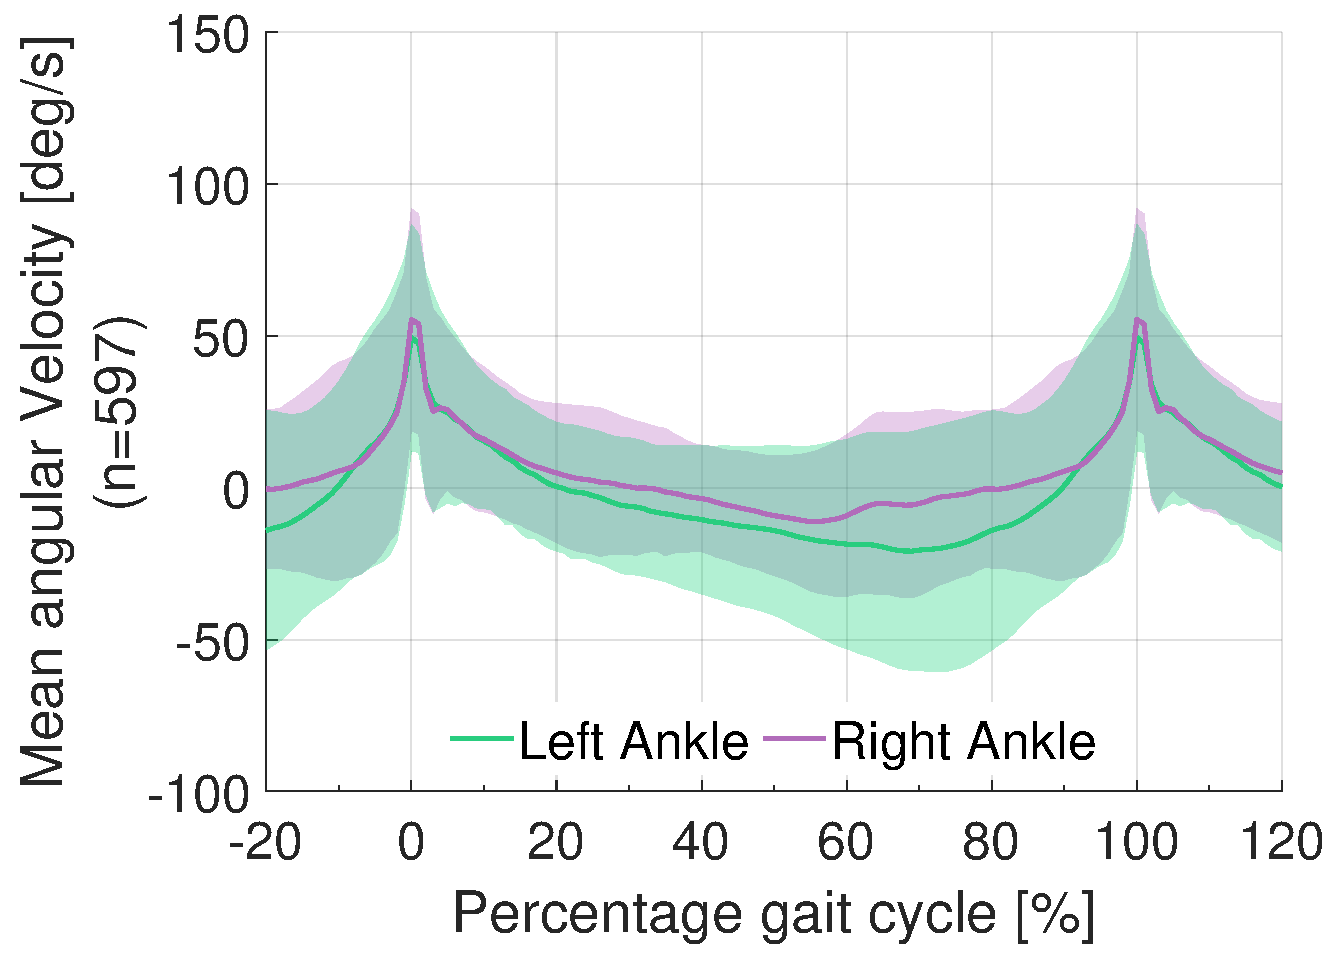
\includegraphics[width=0.275\linewidth]{content/5-Personalisation/Gyro_Trends_For_Targets/ch5_gait_trends_subject_03_activity_stair_up.pdf} &
        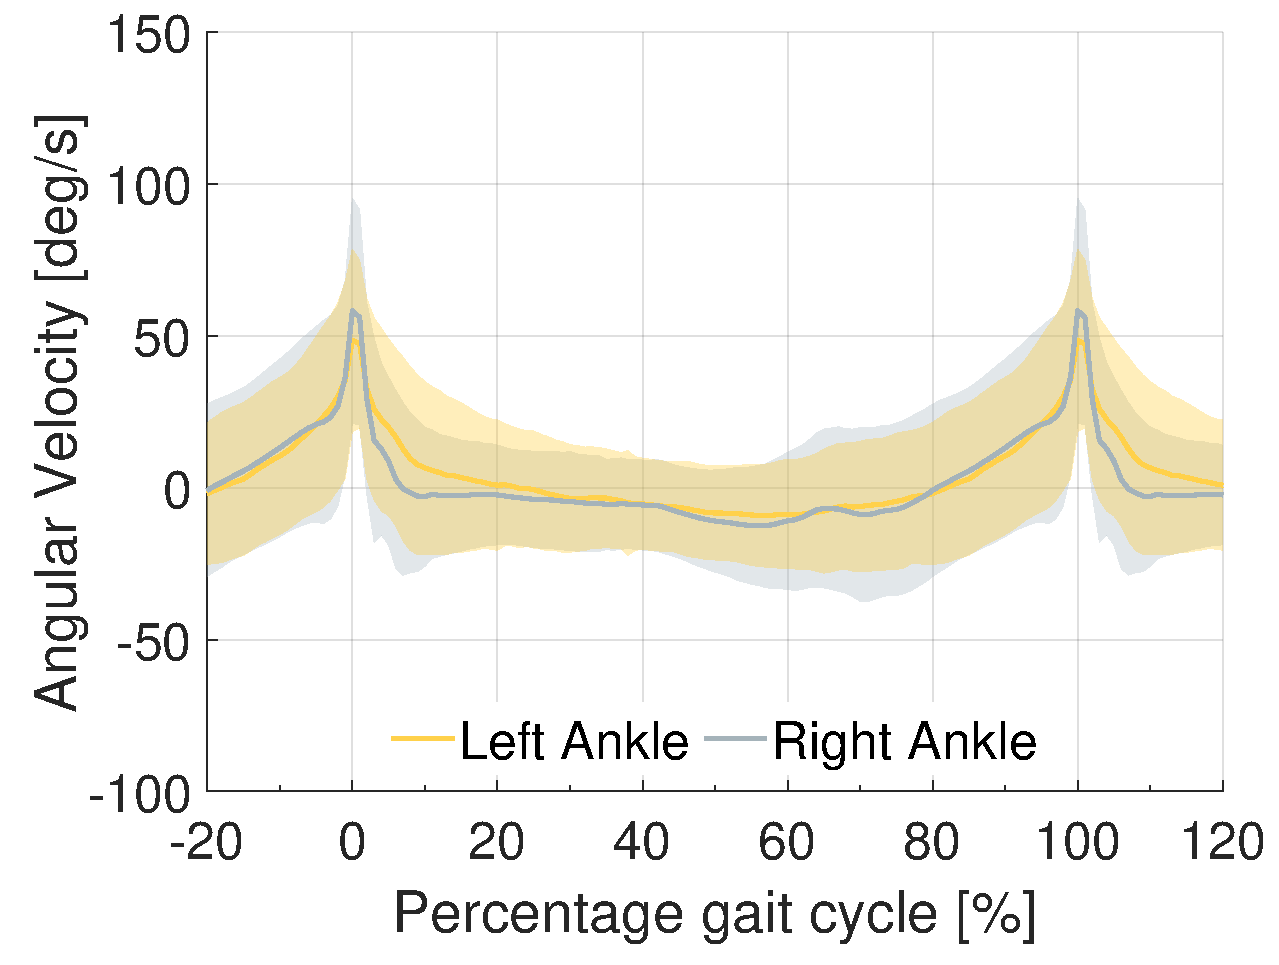
\includegraphics[width=0.275\linewidth]{content/5-Personalisation/Gyro_Trends_For_Targets/ch5_gait_trends_subject_09_activity_stair_up.pdf} \\
        
        \rotatebox{90}{\quad \textbf{\glsentrylong{sd}}} & 
        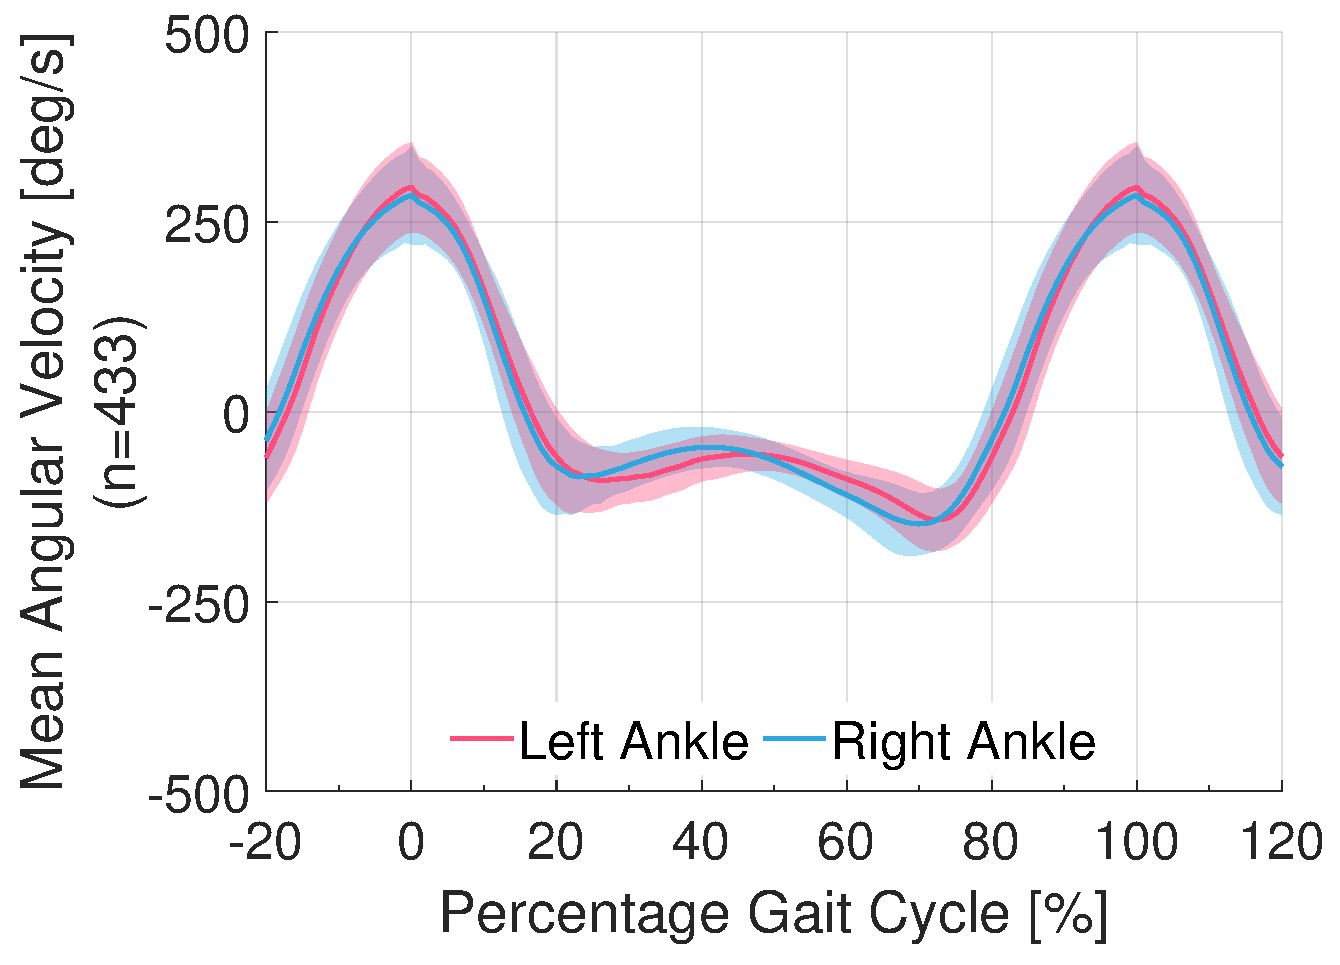
\includegraphics[width=0.275\linewidth]{content/5-Personalisation/Gyro_Trends_For_Targets/ch5_gait_trends_subject_01_activity_stair_down.pdf} & 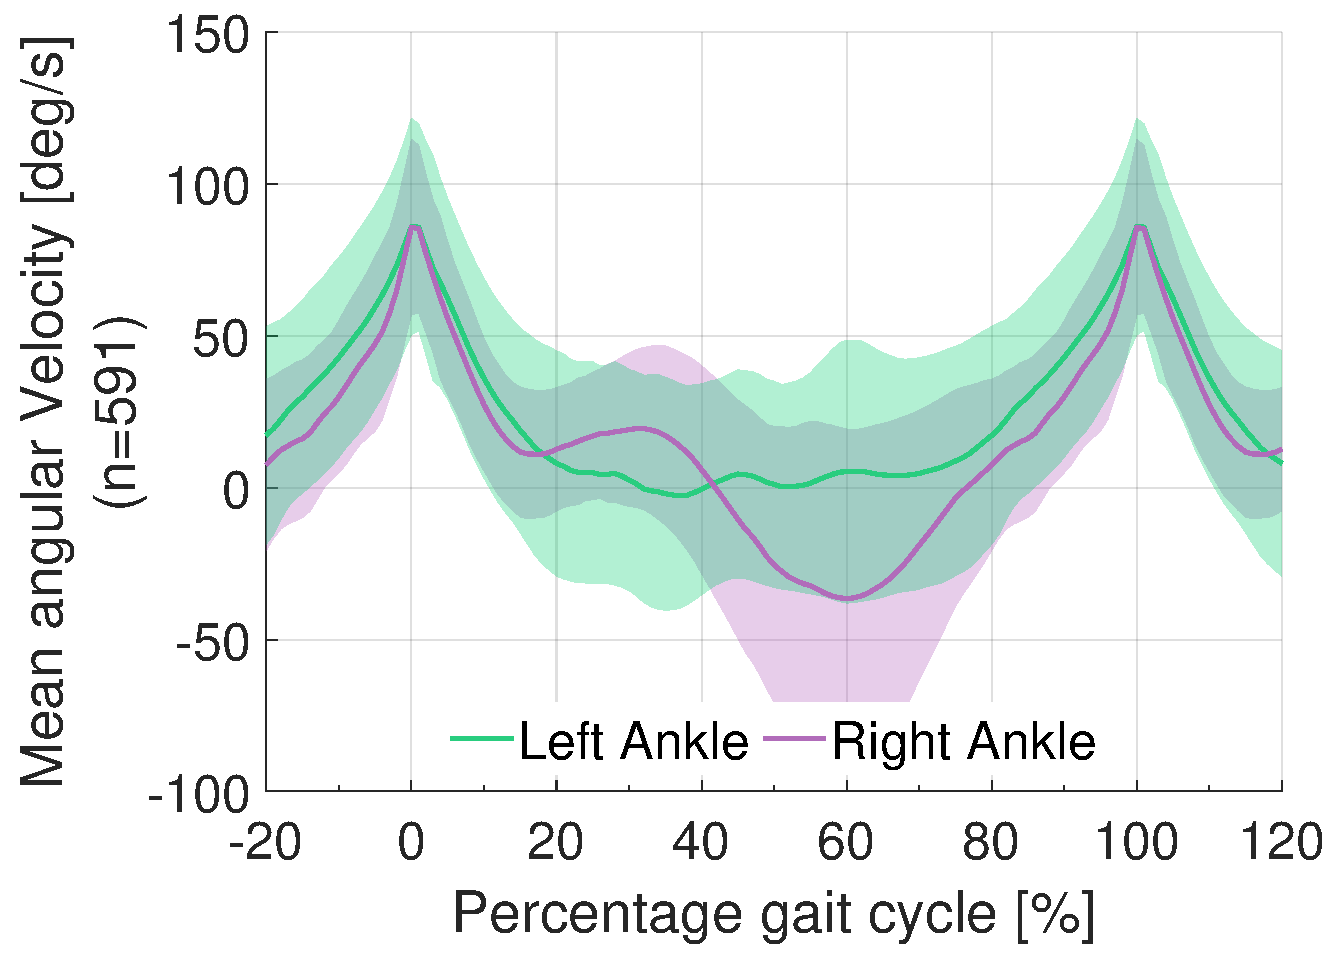
\includegraphics[width=0.275\linewidth]{content/5-Personalisation/Gyro_Trends_For_Targets/ch5_gait_trends_subject_03_activity_stair_down.pdf} &
        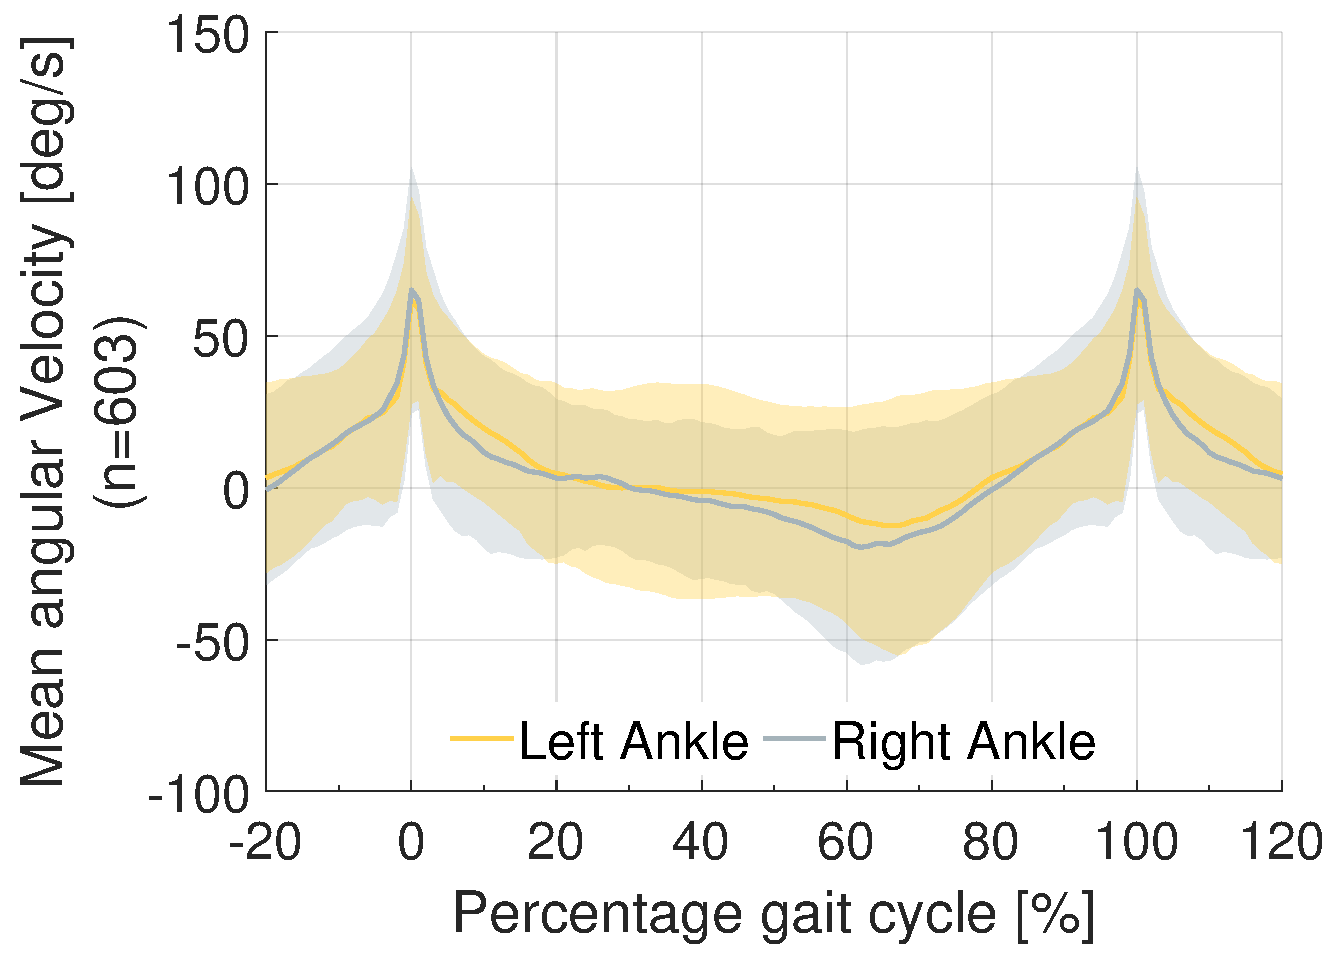
\includegraphics[width=0.275\linewidth]{content/5-Personalisation/Gyro_Trends_For_Targets/ch5_gait_trends_subject_09_activity_stair_down.pdf} \\
    \end{tabular}
    \centering
    
    % \hspace*{1cm}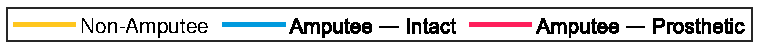
\includegraphics[width=0.7\textwidth]{content/6-Amputee/Gait-Trends/Legend.pdf}
    
    \caption[Angular velocity of the shank in the Saggital Plane during different activities for the three target subject]{Angular velocity of the shank in the Saggital Plane during different activities for the three target subject. The solid line shows the mean angular velocity for all steps recorded for each activity. The filled area represents the standard deviation. 0\% gait cycle is taken as peak swing for simplicity of calculation. The red, green and yellow lines are for the left ankles of Subjects 01, 03 and 09 respectively. The blue, purple and grey lines show the right ankles of Subjects 01, 03 and 09 respectively.}
    \label{fig:ch6_target_subject_gyro_trends}
\end{figure}

%--------------------------------
% Machine learning methods
To perform machine learning on just a single participant a different data division method is required than in the previous work. Instead using participants as the division point. Transitions between activity was used as previously described in \ref{par:methods-per-episode-division}.

What kind of ML model are we going to use?
% TODO: Add in LSTM model being tested
\begin{figure}[htbp]
    \centering
    \includegraphics[width=0.6\textwidth]{example-image-duck}
    \caption{Illustration of LSTM model that is being tested}
    \label{fig:ch5_illustration_of_base_LSTM_model}
\end{figure}

How were general models produced?

How are we going to perform our personalisation/transfer learning
% Train with a mixture of both target and source data
% Re-train a pre-trained model
% Freezing trainable parameters on set layers to 

%---------------------------
% Performance metrics
How are we going to determine performance? Categorical accuracy, Confusion Matrices, F1-Scores
% What would better than the baseline look like. Less data, faster at training, better performance

\begin{figure}[htbp]
    \centering
    \includegraphics[width=0.6\textwidth]{example-image-duck}
    \caption{LSTM Setups for transfer learning}
    \label{fig:ch5_LSTM_model_transfer_learning}
\end{figure}


%-------------------------------------------------------------------------------
\section{Baseline Model Performance}
\label{sec:personalisation-baseline-model-results}
Want to determine a baseline performance that can be achieved using only one individuals data. If performance of new methods does not exceed this value there is no benefit in the methods. Feed in increasing amounts of training data into the training process and see what performance improvements can be seen.

% Training performance vs quantity of data for both subjects
X axis is windows of data per class. Each window is 128 samples long at 100Hz, with a skip value of 3 samples so from 30 seconds per class to 450 seconds per class. Test samples was fixed at 5000 samples for all evaluations - 151 seconds

Figure \ref{fig:ch5_bespoke_mode_classification} shows the classification performance for the three Target subjects for different amounts of target data windows and different sized LSTM networks. Full data tables are available in Appendix \ref{sec:appendix-a-model-performance-bespoke}.

\begin{figure}[p]
    \centering
    \begin{subfigure}[b]{0.9\textwidth}
        \centering
        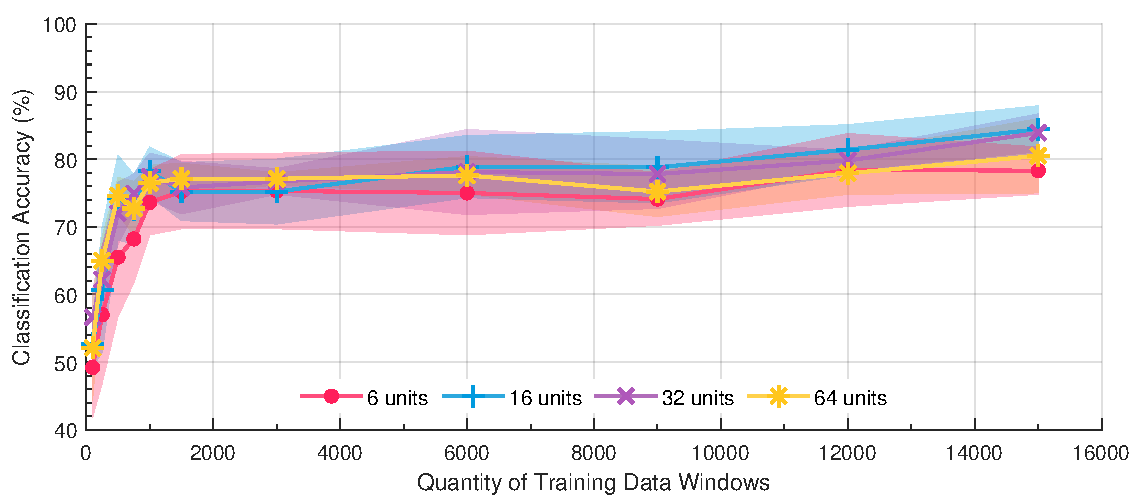
\includegraphics[width=\textwidth]{content/5-Personalisation/Bespoke_Target/ch5_bespoke_target_model_subject_1.pdf}
        \caption{Subject 01}
        \label{fig:ch5_6_unit_bespoke_model}
    \end{subfigure}
    \begin{subfigure}[b]{0.9\textwidth}
        \centering
        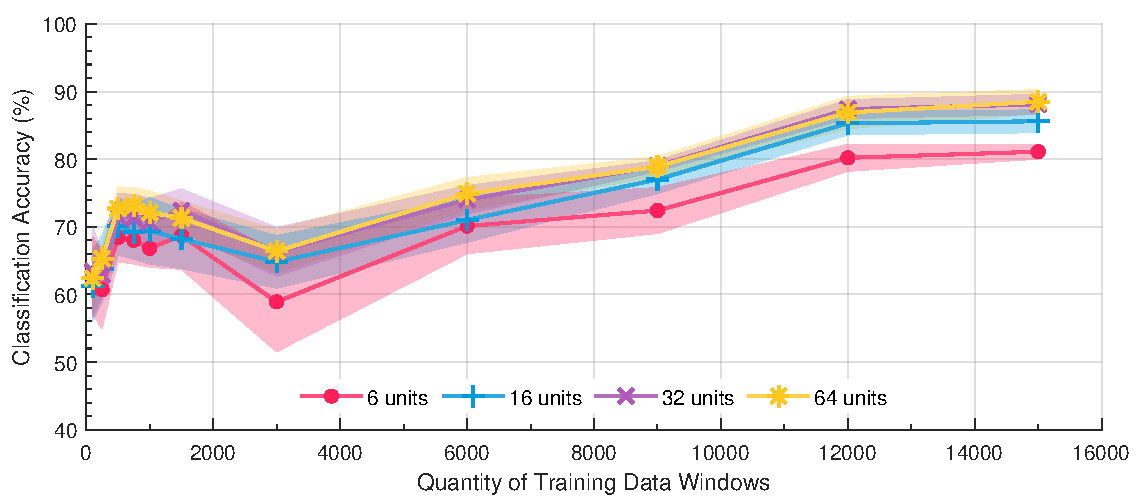
\includegraphics[width=\textwidth]{content/5-Personalisation/Bespoke_Target/ch5_bespoke_target_model_subject_3.pdf}
        \caption{Subject 03}
        \label{fig:ch5_16_unit_bespoke_model}
    \end{subfigure}
    \begin{subfigure}[b]{0.9\textwidth}
        \centering
        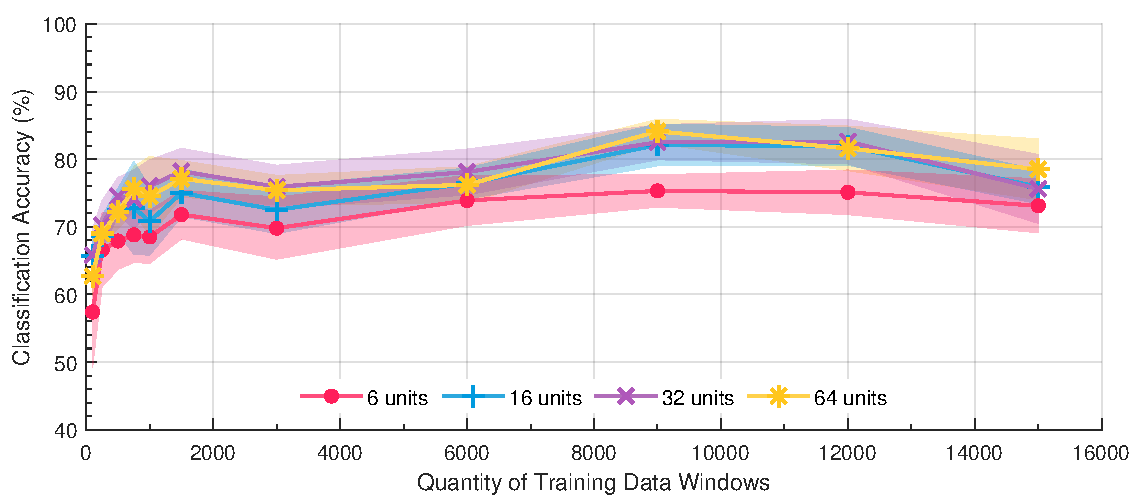
\includegraphics[width=\textwidth]{content/5-Personalisation/Bespoke_Target/ch5_bespoke_target_model_subject_9.pdf}
        \caption{Subject 09}
        \label{fig:ch5_32_unit_bespoke_model}
    \end{subfigure}
    \caption[TODO Caption]{\hl{TODO Caption}}
    \label{fig:ch5_bespoke_mode_classification}
\end{figure}

Maximum performance achieved was 84.4\% for Subject 01, 88.5\% for Subject 03, and 82.6\% for Subject 09.

Performance improves rapidly from 100 to 1500 data samples, there is then a gradual increase in performance for the remaining increases in training windows.

Performance appears to still be increasing when the maximum amount of data was tested. Indicating further data would still improve performance. Not realistic to expose the model to every possible environment that it will need to operate on.

Standard deviation reduces with increasing data windows indicating more consistent performance across the 5 test sets.

Reduction in performance at 3000 samples for Subject 03 is likely due to model exposure to a new environment of data. Performance recovers with increasing amounts of data. Subject 09 also experiences similar drops in performance.

Increasing the number of units in general improved classification performance. This levels off at 32 units. Only the 6 unit model appears to have insufficient learning capacity. 

Increasing the number of units also reduced the number of epochs required to train the models. 

%Why is the model not achieving better performance?
By looking at the confusion matrices it can be seen which classes the models are struggling to identify. Table \ref{tab:ch5-bespoke-mode-confusion-matrix_subject_09} shows confusion matrices for the three targets subjects when the model is presented with test data.

\begin{table}[p]
    \centering
    \caption[Confusion matrix of test data for a 32 unit trained with \hl{x} target data LSTM model]{\hl{TODO: Put in correct values}Confusion matrix of test data for a 32 unit trained with \hl{x} target data LSTM model. (\acrfull{ra}, \acrfull{rd}, \acrfull{sa}, \acrfull{sd})}
    \label{tab:ch5-bespoke-mode-confusion-matrix_subject_09}
    \begin{subtable}{\textwidth}
    \caption{Subject 01}
    \begin{tabularx}{\textwidth}{ccYYYYYY}
        \noalign{\hrule height 1.5pt}
         & & \multicolumn{6}{c}{\textbf{Predicted Classes}} \\
         \hline
         & & WALK & \glsentryshort{ra} & \glsentryshort{rd} & \glsentryshort{sa} & \glsentryshort{sd} & STOP \\
         \multirow{6}{*}{\rotatebox{90}{\textbf{True Classes}}} 
         & WALK               & 100\% & 0 & 0 & 0 & 0 & 0 \\
         & \glsentryshort{ra} & 0 & 98\% & 2\% & 0 & 0 & 0 \\
         & \glsentryshort{rd} & 0 & 0 & 100\% & 0 & 0 & 0 \\
         & \glsentryshort{sa} & 0 & 0 & 0 & 100\% & 0 & 0 \\
         & \glsentryshort{sd} & 0 & 0 & 0 & 0 & 100\% & 0 \\
         & STOP               & 0 & 0 & 0 & 0 & 0 & 100\% \\
         \noalign{\hrule height 1.5pt} \\
    \end{tabularx}
    \end{subtable}
    \begin{subtable}{\textwidth}
    \caption{Subject 03}
    \begin{tabularx}{\textwidth}{ccYYYYYY}
        \noalign{\hrule height 1.5pt}
         & & \multicolumn{6}{c}{\textbf{Predicted Classes}} \\
         \hline
         & & WALK & \glsentryshort{ra} & \glsentryshort{rd} & \glsentryshort{sa} & \glsentryshort{sd} & STOP \\
         \multirow{6}{*}{\rotatebox{90}{\textbf{True Classes}}} 
         & WALK               & 100\% & 0 & 0 & 0 & 0 & 0 \\
         & \glsentryshort{ra} & 0 & 98\% & 2\% & 0 & 0 & 0 \\
         & \glsentryshort{rd} & 0 & 0 & 100\% & 0 & 0 & 0 \\
         & \glsentryshort{sa} & 0 & 0 & 0 & 100\% & 0 & 0 \\
         & \glsentryshort{sd} & 0 & 0 & 0 & 0 & 100\% & 0 \\
         & STOP               & 0 & 0 & 0 & 0 & 0 & 100\% \\
         \noalign{\hrule height 1.5pt} \\
    \end{tabularx}
    \end{subtable}
    \begin{subtable}{\textwidth}
    \caption{Subject 09}
    \begin{tabularx}{\textwidth}{ccYYYYYY}
        \noalign{\hrule height 1.5pt}
         & & \multicolumn{6}{c}{\textbf{Predicted Classes}} \\
         \hline
         & & WALK & \glsentryshort{ra} & \glsentryshort{rd} & \glsentryshort{sa} & \glsentryshort{sd} & STOP \\
         \multirow{6}{*}{\rotatebox{90}{\textbf{True Classes}}} 
         & WALK               & 100\% & 0 & 0 & 0 & 0 & 0 \\
         & \glsentryshort{ra} & 0 & 98\% & 2\% & 0 & 0 & 0 \\
         & \glsentryshort{rd} & 0 & 0 & 100\% & 0 & 0 & 0 \\
         & \glsentryshort{sa} & 0 & 0 & 0 & 100\% & 0 & 0 \\
         & \glsentryshort{sd} & 0 & 0 & 0 & 0 & 100\% & 0 \\
         & STOP               & 0 & 0 & 0 & 0 & 0 & 100\% \\
         \noalign{\hrule height 1.5pt} \\
    \end{tabularx}
    \end{subtable}
\end{table}

Talk about f-scores - indicate poor performance for Walking, Ramp Ascent and Ramp Descent
% Present graph of Learning rate

% Analysis points points
% - Why did subject x perform worse
% - Would more data help?
% - What baseline does this set for our subsequent work


%-------------------------------------------------------------------------------
\section{Model Personalisation}
\label{sec:model-personalisation-results}
% Introductory paragraph
Introductory paragraph
% Aims of this experiment - determine if using additional data from other individuals can improve the performance of a bespoke model

% \subsection{Results and Analysis}
% % Introductory Paragraph

%-------------------------------------------------------------------------------
\subsection{Data Grouping}
Deep learning doesn't lend itself well to establishing similarities between different subjects. Instead attempt to bias the training though varying the proportion of test and training data.

% Fully trained model
% Present performance on this model - Categorical accuracy of training data, learning rate (epochs vs categorical accuracy)
\begin{landscape}
% Subject 01 - classification accuracy for varying source and target data
\begin{table}[p]
    \centering
    \caption[Table of classification accuracy for Subject 01 for a model trained using varying amounts of Source and Target training data]{Table of classification accuracy for Subject 01 for a model trained using varying amounts of Source and Target training data. The cell value represents the percentage classification accuracy $\pm\sigma$. The highest classification accuracy has been highlighted in bold.}
    \ \\
    \label{tab:ch5-mixed-target-and-source-data-subject-01}
    \begin{tabular}{cr| *{7}{C{2cm}}}
        \noalign{\hrule height 1.5pt}
         & & \multicolumn{7}{c}{\textbf{Source Training Windows}}\\
         & & 100 & 250 & 500 & 750 & 1000 & 1500 & 3000 \\
         \hline
         
         \multirow{11}{*}{\rotatebox{90}{\parbox{5.3cm}{\centering\textbf{Target Training Windows}}}}
         
         & 100 & $0.601{\scriptscriptstyle\pm0.07}$ & $0.630{\scriptscriptstyle\pm0.06}$ & $0.587{\scriptscriptstyle\pm0.05}$ & $0.620{\scriptscriptstyle\pm0.02}$ & $0.572{\scriptscriptstyle\pm0.06}$ & $0.587{\scriptscriptstyle\pm0.04}$ & $0.592{\scriptscriptstyle\pm0.04}$ \\
         & 250 & $0.609{\scriptscriptstyle\pm0.08}$ & $0.696{\scriptscriptstyle\pm0.04}$ & $0.643{\scriptscriptstyle\pm0.05}$ & $0.649{\scriptscriptstyle\pm0.06}$ & $0.631{\scriptscriptstyle\pm0.06}$ & $0.630{\scriptscriptstyle\pm0.08}$ & $0.651{\scriptscriptstyle\pm0.02}$ \\
         & 500   & $0.743{\scriptscriptstyle\pm0.02}$ & $0.713{\scriptscriptstyle\pm0.04}$ & $0.741{\scriptscriptstyle\pm0.02}$ & $0.731{\scriptscriptstyle\pm0.04}$ & $0.711{\scriptscriptstyle\pm0.04}$ & $0.727{\scriptscriptstyle\pm0.03}$ & $0.737{\scriptscriptstyle\pm0.04}$ \\
         & 750  & $0.736{\scriptscriptstyle\pm0.03}$ & $0.708{\scriptscriptstyle\pm0.06}$ & $0.721{\scriptscriptstyle\pm0.03}$ & $0.747{\scriptscriptstyle\pm0.02}$ & $0.731{\scriptscriptstyle\pm0.03}$ & $0.735{\scriptscriptstyle\pm0.04}$ & $0.782{\scriptscriptstyle\pm0.03}$ \\
         & 1000 & $0.769{\scriptscriptstyle\pm0.02}$ & $0.782{\scriptscriptstyle\pm0.04}$ & $0.748{\scriptscriptstyle\pm0.01}$ & $0.768{\scriptscriptstyle\pm0.02}$ & $0.768{\scriptscriptstyle\pm0.05}$ & $0.775{\scriptscriptstyle\pm0.03}$ & $0.772{\scriptscriptstyle\pm0.02}$ \\
         & 1500  & $0.769{\scriptscriptstyle\pm0.05}$ & $0.778{\scriptscriptstyle\pm0.02}$ & $0.781{\scriptscriptstyle\pm0.04}$ & $0.758{\scriptscriptstyle\pm0.02}$ & $0.757{\scriptscriptstyle\pm0.01}$ & $0.793{\scriptscriptstyle\pm0.05}$ & $0.770{\scriptscriptstyle\pm0.04}$ \\
         & 3000  & $0.774{\scriptscriptstyle\pm0.04}$ & $0.756{\scriptscriptstyle\pm0.05}$ & $0.787{\scriptscriptstyle\pm0.02}$ & $0.730{\scriptscriptstyle\pm0.03}$ & $0.741{\scriptscriptstyle\pm0.02}$ & $0.786{\scriptscriptstyle\pm0.02}$ & $0.776{\scriptscriptstyle\pm0.02}$ \\
         & 6000  & $0.799{\scriptscriptstyle\pm0.06}$ & $0.797{\scriptscriptstyle\pm0.03}$ & $0.764{\scriptscriptstyle\pm0.06}$ & $0.773{\scriptscriptstyle\pm0.04}$ & $0.754{\scriptscriptstyle\pm0.03}$ & $0.774{\scriptscriptstyle\pm0.02}$ & $0.792{\scriptscriptstyle\pm0.05}$ \\
         & 9000  & $0.749{\scriptscriptstyle\pm0.04}$ & $0.781{\scriptscriptstyle\pm0.05}$ & $0.785{\scriptscriptstyle\pm0.04}$ & $0.767{\scriptscriptstyle\pm0.06}$ & $0.743{\scriptscriptstyle\pm0.03}$ & $0.754{\scriptscriptstyle\pm0.03}$ & $0.752{\scriptscriptstyle\pm0.04}$ \\
         & 12000 & $0.805{\scriptscriptstyle\pm0.03}$ & $0.754{\scriptscriptstyle\pm0.07}$ & $0.798{\scriptscriptstyle\pm0.04}$ & $0.782{\scriptscriptstyle\pm0.05}$ & $0.816{\scriptscriptstyle\pm0.02}$ & $0.777{\scriptscriptstyle\pm0.04}$ & $0.794{\scriptscriptstyle\pm0.02}$ \\
         & 15000 & $0.855{\scriptscriptstyle\pm0.03}$ & $0.822{\scriptscriptstyle\pm0.04}$ & $0.848{\scriptscriptstyle\pm0.02}$ & $\mathbf{0.861{\scriptscriptstyle\pm0.02}}$ & $0.836{\scriptscriptstyle\pm0.05}$ & $0.829{\scriptscriptstyle\pm0.02}$ & $0.833{\scriptscriptstyle\pm0.02}$ \\
         \noalign{\hrule height 1.5pt}
    \end{tabular}
    \ \\ \vspace{0.5cm}
    \begin{tabular}{cr| *{4}{C{2cm}}}
        \noalign{\hrule height 1.5pt}
         & & \multicolumn{4}{c}{\textbf{Source Training Windows}}\\
         & & 6000 & 9000 & 12000 & 15000 \\
         \hline
         \multirow{11}{*}{\rotatebox{90}{\parbox{5.3cm}{\centering\textbf{Target Training Windows}}}}
         
         & 100 & $0.590{\scriptscriptstyle\pm0.07}$ & $0.584{\scriptscriptstyle\pm0.03}$ & $0.618{\scriptscriptstyle\pm0.03}$ & $0.593{\scriptscriptstyle\pm0.02}$ \\
         
        & 250 & $0.670{\scriptscriptstyle\pm0.02}$ & $0.617{\scriptscriptstyle\pm0.04}$ & $0.661{\scriptscriptstyle\pm0.05}$ & $0.685{\scriptscriptstyle\pm0.04}$ \\
        
        & 500 & $0.713{\scriptscriptstyle\pm0.06}$ & $0.731{\scriptscriptstyle\pm0.02}$ & $0.754{\scriptscriptstyle\pm0.03}$ & $0.716{\scriptscriptstyle\pm0.05}$ \\
        
        & 750 & $0.746{\scriptscriptstyle\pm0.02}$ & $0.729{\scriptscriptstyle\pm0.03}$ & $0.782{\scriptscriptstyle\pm0.03}$ & $0.743{\scriptscriptstyle\pm0.03}$ \\
        
        & 1000 & $0.774{\scriptscriptstyle\pm0.04}$ & $0.748{\scriptscriptstyle\pm0.02}$ & $0.761{\scriptscriptstyle\pm0.03}$ & $0.771{\scriptscriptstyle\pm0.01}$ \\
        
        & 1500 & $0.789{\scriptscriptstyle\pm0.04}$ & $0.786{\scriptscriptstyle\pm0.05}$ & $0.746{\scriptscriptstyle\pm0.04}$ & $0.731{\scriptscriptstyle\pm0.02}$ \\
        
        & 3000 & $0.770{\scriptscriptstyle\pm0.01}$ & $0.764{\scriptscriptstyle\pm0.02}$ & $0.776{\scriptscriptstyle\pm0.01}$ & $0.755{\scriptscriptstyle\pm0.05}$ \\ 
        
        & 6000 & $0.794{\scriptscriptstyle\pm0.01}$ & $0.805{\scriptscriptstyle\pm0.03}$ & $0.763{\scriptscriptstyle\pm0.06}$ & $0.775{\scriptscriptstyle\pm0.03}$ \\
        
        & 9000 & $0.765{\scriptscriptstyle\pm0.04}$ & $0.751{\scriptscriptstyle\pm0.04}$ & $0.776{\scriptscriptstyle\pm0.06}$ & $0.761{\scriptscriptstyle\pm0.03}$ \\
        
        & 12000 & $0.789{\scriptscriptstyle\pm0.04}$ & $0.813{\scriptscriptstyle\pm0.04}$ & $0.773{\scriptscriptstyle\pm0.02}$ & $0.801{\scriptscriptstyle\pm0.01}$ \\
        
        & 15000 & $0.846{\scriptscriptstyle\pm0.04}$ & $0.846{\scriptscriptstyle\pm0.01}$ & $0.843{\scriptscriptstyle\pm0.02}$ & $0.852{\scriptscriptstyle\pm0.01}$ \\
        
        \noalign{\hrule height 1.5pt}
    \end{tabular}
\end{table}

% Subject 03 - classification accuracy for varying source and target data
\begin{table}[p]
    \centering
    \caption[Table of classification accuracy for Subject 03 for a model trained using varying amounts of Source and Target training data]{Table of classification accuracy for Subject 03 for a model trained using varying amounts of Source and Target training data. The cell value represents the percentage classification accuracy $\pm\sigma$. The highest classification accuracy has been highlighted in bold.}
    \ \\
    \label{tab:ch5-mixed-target-and-source-data-subject-03}
    \begin{tabular}{cr| *{7}{C{2cm}}}
        \noalign{\hrule height 1.5pt}
         & & \multicolumn{7}{c}{\textbf{Source Training Windows}}\\
         & & 100 & 250 & 500 & 750 & 1000 & 1500 & 3000 \\
         \hline
         
         \multirow{11}{*}{\rotatebox{90}{\parbox{5.3cm}{\centering\textbf{Target Training Windows}}}}
         
        & 100 & $0.635{\scriptscriptstyle\pm0.05}$ & $0.682{\scriptscriptstyle\pm0.01}$ & $0.662{\scriptscriptstyle\pm0.02}$ & $0.670{\scriptscriptstyle\pm0.05}$ & $0.658{\scriptscriptstyle\pm0.04}$ & $0.635{\scriptscriptstyle\pm0.06}$ & $0.652{\scriptscriptstyle\pm0.02}$ \\
        & 250 & $0.662{\scriptscriptstyle\pm0.06}$ & $0.687{\scriptscriptstyle\pm0.02}$ & $0.653{\scriptscriptstyle\pm0.03}$ & $0.675{\scriptscriptstyle\pm0.04}$ & $0.629{\scriptscriptstyle\pm0.04}$ & $0.673{\scriptscriptstyle\pm0.04}$ & $0.671{\scriptscriptstyle\pm0.05}$ \\
        & 500 & $0.707{\scriptscriptstyle\pm0.06}$ & $0.724{\scriptscriptstyle\pm0.03}$ & $0.698{\scriptscriptstyle\pm0.05}$ & $0.700{\scriptscriptstyle\pm0.02}$ & $0.713{\scriptscriptstyle\pm0.03}$ & $0.724{\scriptscriptstyle\pm0.04}$ & $0.695{\scriptscriptstyle\pm0.02}$ \\
        & 750 & $0.698{\scriptscriptstyle\pm0.03}$ & $0.726{\scriptscriptstyle\pm0.02}$ & $0.741{\scriptscriptstyle\pm0.01}$ & $0.682{\scriptscriptstyle\pm0.01}$ & $0.706{\scriptscriptstyle\pm0.04}$ & $0.664{\scriptscriptstyle\pm0.04}$ & $0.696{\scriptscriptstyle\pm0.03}$ \\
        & 1000 & $0.693{\scriptscriptstyle\pm0.05}$ & $0.687{\scriptscriptstyle\pm0.04}$ & $0.717{\scriptscriptstyle\pm0.02}$ & $0.680{\scriptscriptstyle\pm0.04}$ & $0.710{\scriptscriptstyle\pm0.03}$ & $0.733{\scriptscriptstyle\pm0.03}$ & $0.688{\scriptscriptstyle\pm0.04}$ \\
        & 1500 & $0.706{\scriptscriptstyle\pm0.04}$ & $0.703{\scriptscriptstyle\pm0.03}$ & $0.696{\scriptscriptstyle\pm0.04}$ & $0.709{\scriptscriptstyle\pm0.02}$ & $0.689{\scriptscriptstyle\pm0.04}$ & $0.700{\scriptscriptstyle\pm0.08}$ & $0.703{\scriptscriptstyle\pm0.05}$ \\
        & 3000 & $0.670{\scriptscriptstyle\pm0.02}$ & $0.651{\scriptscriptstyle\pm0.04}$ & $0.671{\scriptscriptstyle\pm0.03}$ & $0.655{\scriptscriptstyle\pm0.04}$ & $0.688{\scriptscriptstyle\pm0.02}$ & $0.672{\scriptscriptstyle\pm0.02}$ & $0.670{\scriptscriptstyle\pm0.03}$ \\
        & 6000 & $0.752{\scriptscriptstyle\pm0.02}$ & $0.737{\scriptscriptstyle\pm0.00}$ & $0.764{\scriptscriptstyle\pm0.01}$ & $0.744{\scriptscriptstyle\pm0.01}$ & $0.751{\scriptscriptstyle\pm0.02}$ & $0.744{\scriptscriptstyle\pm0.02}$ & $0.735{\scriptscriptstyle\pm0.04}$ \\
        & 9000 & $0.798{\scriptscriptstyle\pm0.01}$ & $0.780{\scriptscriptstyle\pm0.01}$ & $0.780{\scriptscriptstyle\pm0.03}$ & $0.767{\scriptscriptstyle\pm0.01}$ & $0.786{\scriptscriptstyle\pm0.02}$ & $0.781{\scriptscriptstyle\pm0.01}$ & $0.778{\scriptscriptstyle\pm0.03}$ \\
        & 12000 & $0.876{\scriptscriptstyle\pm0.01}$ & $0.858{\scriptscriptstyle\pm0.01}$ & $0.868{\scriptscriptstyle\pm0.01}$ & $0.873{\scriptscriptstyle\pm0.01}$ & $0.861{\scriptscriptstyle\pm0.02}$ & $0.874{\scriptscriptstyle\pm0.02}$ & $0.867{\scriptscriptstyle\pm0.01}$ \\
        & 15000 & $0.871{\scriptscriptstyle\pm0.01}$ & $0.885{\scriptscriptstyle\pm0.01}$ & $0.880{\scriptscriptstyle\pm0.01}$ & $0.873{\scriptscriptstyle\pm0.01}$ & $0.883{\scriptscriptstyle\pm0.01}$ & $0.884{\scriptscriptstyle\pm0.02}$ & $0.879{\scriptscriptstyle\pm0.01}$ \\

         \noalign{\hrule height 1.5pt}
    \end{tabular}
    \ \\ \vspace{0.5cm}
    \begin{tabular}{cr| *{4}{C{2cm}}}
        \noalign{\hrule height 1.5pt}
        & & \multicolumn{4}{c}{\textbf{Source Training Windows}}\\
        & & 6000 & 9000 & 12000 & 15000 \\
        \hline
        \multirow{11}{*}{\rotatebox{90}{\parbox{5.3cm}{\centering\textbf{Target Training Windows}}}}
         
        & 100 & $0.649{\scriptscriptstyle\pm0.04}$ & $0.648{\scriptscriptstyle\pm0.03}$ & $0.627{\scriptscriptstyle\pm0.05}$ & $0.683{\scriptscriptstyle\pm0.04}$ \\
        & 250 & $0.630{\scriptscriptstyle\pm0.03}$ & $0.635{\scriptscriptstyle\pm0.03}$ & $0.648{\scriptscriptstyle\pm0.08}$ & $0.670{\scriptscriptstyle\pm0.04}$ \\
        & 500 & $0.723{\scriptscriptstyle\pm0.01}$ & $0.714{\scriptscriptstyle\pm0.01}$ & $0.696{\scriptscriptstyle\pm0.04}$ & $0.671{\scriptscriptstyle\pm0.05}$ \\
        & 750 & $0.716{\scriptscriptstyle\pm0.01}$ & $0.727{\scriptscriptstyle\pm0.02}$ & $0.717{\scriptscriptstyle\pm0.04}$ & $0.730{\scriptscriptstyle\pm0.03}$ \\
        & 1000 & $0.729{\scriptscriptstyle\pm0.02}$ & $0.687{\scriptscriptstyle\pm0.05}$ & $0.715{\scriptscriptstyle\pm0.04}$ & $0.709{\scriptscriptstyle\pm0.02}$ \\
        & 1500 & $0.728{\scriptscriptstyle\pm0.03}$ & $0.705{\scriptscriptstyle\pm0.05}$ & $0.729{\scriptscriptstyle\pm0.02}$ & $0.728{\scriptscriptstyle\pm0.01}$ \\
        & 3000 & $0.639{\scriptscriptstyle\pm0.03}$ & $0.688{\scriptscriptstyle\pm0.03}$ & $0.686{\scriptscriptstyle\pm0.02}$ & $0.675{\scriptscriptstyle\pm0.01}$ \\
        & 6000 & $0.725{\scriptscriptstyle\pm0.02}$ & $0.743{\scriptscriptstyle\pm0.02}$ & $0.753{\scriptscriptstyle\pm0.04}$ & $0.757{\scriptscriptstyle\pm0.02}$ \\
        & 9000 & $0.782{\scriptscriptstyle\pm0.02}$ & $0.788{\scriptscriptstyle\pm0.01}$ & $0.789{\scriptscriptstyle\pm0.02}$ & $0.790{\scriptscriptstyle\pm0.01}$ \\
        & 12000 & $0.864{\scriptscriptstyle\pm0.03}$ & $0.855{\scriptscriptstyle\pm0.01}$ & $0.870{\scriptscriptstyle\pm0.02}$ & $0.854{\scriptscriptstyle\pm0.02}$ \\
        & 15000 & $0.888{\scriptscriptstyle\pm0.02}$ & $\mathbf{0.897{\scriptscriptstyle\pm0.01}}$ & $0.871{\scriptscriptstyle\pm0.02}$ & $0.882{\scriptscriptstyle\pm0.01}$ \\
                
        \noalign{\hrule height 1.5pt}
    \end{tabular}
\end{table}

% Subject 09 - classification accuracy for varying source and target data
\begin{table}[p]
    \centering
    \caption[Table of classification accuracy for Subject 09 for a model trained using varying amounts of Source and Target training data]{Table of classification accuracy for Subject 09 for a model trained using varying amounts of Source and Target training data. The cell value represents the percentage classification accuracy $\pm\sigma$. The highest classification accuracy has been highlighted in bold.}
    \ \\
    \label{tab:ch5-mixed-target-and-source-data-subject-09}
    \begin{tabular}{cr| *{7}{C{2cm}}}
        \noalign{\hrule height 1.5pt}
         & & \multicolumn{7}{c}{\textbf{Source Training Windows}}\\
         & & 100 & 250 & 500 & 750 & 1000 & 1500 & 3000 \\
         \hline
         
         \multirow{11}{*}{\rotatebox{90}{\parbox{5.3cm}{\centering\textbf{Target Training Windows}}}}
         
        & 100 & $0.648{\scriptscriptstyle\pm0.02}$ & $0.696{\scriptscriptstyle\pm0.02}$ & $0.675{\scriptscriptstyle\pm0.03}$ & $0.686{\scriptscriptstyle\pm0.06}$ & $0.695{\scriptscriptstyle\pm0.05}$ & $0.683{\scriptscriptstyle\pm0.03}$ & $0.679{\scriptscriptstyle\pm0.03}$ \\
        & 250 & $0.710{\scriptscriptstyle\pm0.02}$ & $0.727{\scriptscriptstyle\pm0.03}$ & $0.719{\scriptscriptstyle\pm0.04}$ & $0.739{\scriptscriptstyle\pm0.04}$ & $0.722{\scriptscriptstyle\pm0.02}$ & $0.711{\scriptscriptstyle\pm0.03}$ & $0.754{\scriptscriptstyle\pm0.03}$ \\
        & 500 & $0.736{\scriptscriptstyle\pm0.02}$ & $0.727{\scriptscriptstyle\pm0.05}$ & $0.740{\scriptscriptstyle\pm0.04}$ & $0.747{\scriptscriptstyle\pm0.05}$ & $0.733{\scriptscriptstyle\pm0.04}$ & $0.724{\scriptscriptstyle\pm0.02}$ & $0.752{\scriptscriptstyle\pm0.05}$ \\
        & 750 & $0.748{\scriptscriptstyle\pm0.06}$ & $0.755{\scriptscriptstyle\pm0.03}$ & $0.744{\scriptscriptstyle\pm0.02}$ & $0.749{\scriptscriptstyle\pm0.02}$ & $0.758{\scriptscriptstyle\pm0.05}$ & $0.749{\scriptscriptstyle\pm0.05}$ & $0.706{\scriptscriptstyle\pm0.05}$ \\
        & 1000 & $0.758{\scriptscriptstyle\pm0.04}$ & $0.761{\scriptscriptstyle\pm0.03}$ & $0.757{\scriptscriptstyle\pm0.01}$ & $0.768{\scriptscriptstyle\pm0.03}$ & $0.757{\scriptscriptstyle\pm0.03}$ & $0.755{\scriptscriptstyle\pm0.04}$ & $0.749{\scriptscriptstyle\pm0.04}$ \\
        & 1500 & $0.784{\scriptscriptstyle\pm0.03}$ & $0.790{\scriptscriptstyle\pm0.04}$ & $0.797{\scriptscriptstyle\pm0.03}$ & $0.791{\scriptscriptstyle\pm0.03}$ & $0.775{\scriptscriptstyle\pm0.05}$ & $0.768{\scriptscriptstyle\pm0.04}$ & $0.774{\scriptscriptstyle\pm0.02}$ \\
        & 3000 & $0.738{\scriptscriptstyle\pm0.04}$ & $0.746{\scriptscriptstyle\pm0.03}$ & $0.756{\scriptscriptstyle\pm0.03}$ & $0.754{\scriptscriptstyle\pm0.06}$ & $0.769{\scriptscriptstyle\pm0.04}$ & $0.759{\scriptscriptstyle\pm0.04}$ & $0.735{\scriptscriptstyle\pm0.04}$ \\
        & 6000 & $0.769{\scriptscriptstyle\pm0.03}$ & $0.755{\scriptscriptstyle\pm0.02}$ & $0.769{\scriptscriptstyle\pm0.04}$ & $0.765{\scriptscriptstyle\pm0.03}$ & $0.772{\scriptscriptstyle\pm0.03}$ & $0.761{\scriptscriptstyle\pm0.02}$ & $0.761{\scriptscriptstyle\pm0.01}$ \\
        & 9000 & $0.816{\scriptscriptstyle\pm0.02}$ & $\mathbf{0.864{\scriptscriptstyle\pm0.02}}$ & $0.834{\scriptscriptstyle\pm0.02}$ & $0.842{\scriptscriptstyle\pm0.02}$ & $0.836{\scriptscriptstyle\pm0.01}$ & $0.845{\scriptscriptstyle\pm0.03}$ & $0.832{\scriptscriptstyle\pm0.04}$ \\
        & 12000 & $0.839{\scriptscriptstyle\pm0.04}$ & $0.811{\scriptscriptstyle\pm0.03}$ & $0.846{\scriptscriptstyle\pm0.02}$ & $0.808{\scriptscriptstyle\pm0.04}$ & $0.810{\scriptscriptstyle\pm0.02}$ & $0.813{\scriptscriptstyle\pm0.02}$ & $0.826{\scriptscriptstyle\pm0.05}$ \\
        & 15000 & $0.783{\scriptscriptstyle\pm0.03}$ & $0.745{\scriptscriptstyle\pm0.02}$ & $0.753{\scriptscriptstyle\pm0.03}$ & $0.760{\scriptscriptstyle\pm0.04}$ & $0.792{\scriptscriptstyle\pm0.05}$ & $0.772{\scriptscriptstyle\pm0.05}$ & $0.779{\scriptscriptstyle\pm0.05}$ \\

         \noalign{\hrule height 1.5pt}
    \end{tabular}
    \ \\ \vspace{0.5cm}
    \begin{tabular}{cr| *{4}{C{2cm}}}
        \noalign{\hrule height 1.5pt}
        & & \multicolumn{4}{c}{\textbf{Source Training Windows}}\\
        & & 6000 & 9000 & 12000 & 15000 \\
        \hline
        \multirow{11}{*}{\rotatebox{90}{\parbox{5.3cm}{\centering\textbf{Target Training Windows}}}}
         
        & 100 & $0.667{\scriptscriptstyle\pm0.02}$ & $0.693{\scriptscriptstyle\pm0.02}$ & $0.691{\scriptscriptstyle\pm0.02}$ & $0.671{\scriptscriptstyle\pm0.05}$ \\
        & 250 & $0.714{\scriptscriptstyle\pm0.03}$ & $0.727{\scriptscriptstyle\pm0.02}$ & $0.736{\scriptscriptstyle\pm0.05}$ & $0.699{\scriptscriptstyle\pm0.04}$ \\
        & 500 & $0.755{\scriptscriptstyle\pm0.04}$ & $0.713{\scriptscriptstyle\pm0.03}$ & $0.743{\scriptscriptstyle\pm0.06}$ & $0.723{\scriptscriptstyle\pm0.03}$ \\
        & 750 & $0.762{\scriptscriptstyle\pm0.02}$ & $0.740{\scriptscriptstyle\pm0.03}$ & $0.746{\scriptscriptstyle\pm0.02}$ & $0.721{\scriptscriptstyle\pm0.04}$ \\
        & 1000 & $0.768{\scriptscriptstyle\pm0.02}$ & $0.726{\scriptscriptstyle\pm0.03}$ & $0.762{\scriptscriptstyle\pm0.02}$ & $0.738{\scriptscriptstyle\pm0.06}$ \\
        & 1500 & $0.779{\scriptscriptstyle\pm0.02}$ & $0.755{\scriptscriptstyle\pm0.05}$ & $0.771{\scriptscriptstyle\pm0.04}$ & $0.767{\scriptscriptstyle\pm0.05}$ \\
        & 3000 & $0.766{\scriptscriptstyle\pm0.02}$ & $0.765{\scriptscriptstyle\pm0.03}$ & $0.767{\scriptscriptstyle\pm0.05}$ & $0.760{\scriptscriptstyle\pm0.01}$ \\
        & 6000 & $0.775{\scriptscriptstyle\pm0.04}$ & $0.788{\scriptscriptstyle\pm0.05}$ & $0.762{\scriptscriptstyle\pm0.02}$ & $0.774{\scriptscriptstyle\pm0.03}$ \\
        & 9000 & $0.838{\scriptscriptstyle\pm0.02}$ & $0.840{\scriptscriptstyle\pm0.04}$ & $0.831{\scriptscriptstyle\pm0.02}$ & $0.836{\scriptscriptstyle\pm0.01}$ \\
        & 12000 & $0.827{\scriptscriptstyle\pm0.02}$ & $0.822{\scriptscriptstyle\pm0.05}$ & $0.822{\scriptscriptstyle\pm0.02}$ & $0.828{\scriptscriptstyle\pm0.03}$ \\
        & 15000 & $0.756{\scriptscriptstyle\pm0.06}$ & $0.762{\scriptscriptstyle\pm0.04}$ & $0.766{\scriptscriptstyle\pm0.04}$ & $0.752{\scriptscriptstyle\pm0.03}$ \\

        \noalign{\hrule height 1.5pt}
    \end{tabular}
\end{table}
\end{landscape}


%-------------------------------------------------------------------------------
\subsection{Transfer Learning}
% Present results of test subject before bespoke testing - confusion matrix, categorical accuracy
The average accuracy for the 5 models before retraining was.
Subject 01 $76.5\%\pm3.1$, Subject 03 $81.5\%\pm4.3$ and Subject 09 $65.8\%\pm2.7$


% Present results of test subject after bespoke testing - confusion matrix, categorical accuracy, epochs vs categorical accuracy

% Analyse performance of this methods - model has not learning capacity left - need to train the pre-trained model less

% Use a range of different stopping points for the model
%Which method is used - what is the predicted performance improvement?
% Repeat for different pre-trained models, based on methods presented in the methodology section
\begin{figure}[htbp]
    \centering
    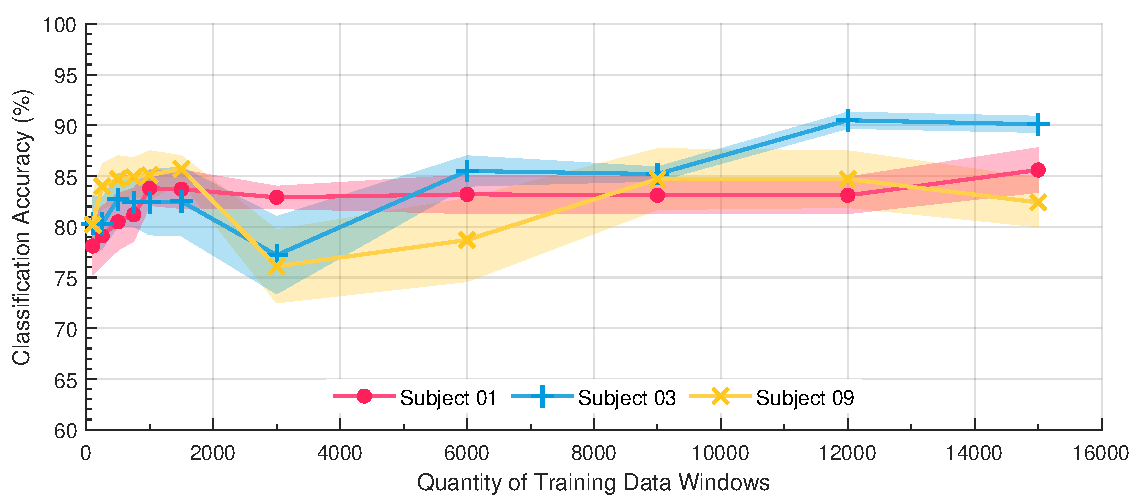
\includegraphics[width=\textwidth]{content/5-Personalisation/ch5_pre_trained_model_accuracy.pdf}
    \caption[Retraining a pre-trained LSTM model]{\hl{Retraining a pre-trained LSTM model}}
    \label{fig:ch5_pretrained_model}
\end{figure}


% Mixed training data
% something akin to k-fold for time varying data (General Data set -> Individual Data set -> General Data set -> Individual Data set)

% Freezing individual layers - Illustration of which layers are frozen
%--------------------------------------------------------
\begin{figure}[htbp]
    \centering
    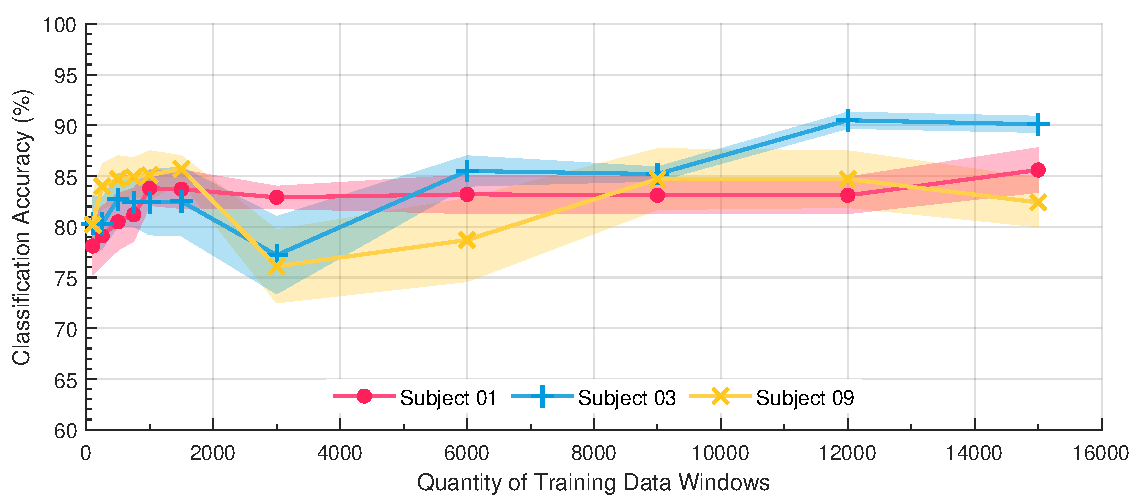
\includegraphics[width=0.95\textwidth]{content/5-Personalisation/ch5_frozen_dense_layer_accuracy.pdf}
    \caption[Retraining a pre-trained LSTM model]{Retraining a pre-trained LSTM model - frozen dense layer}
    \label{fig:ch5_freezing_dense_layer}
\end{figure}


%-------------------------------------------------------------------------------
\begin{figure}[htbp]
    \centering
    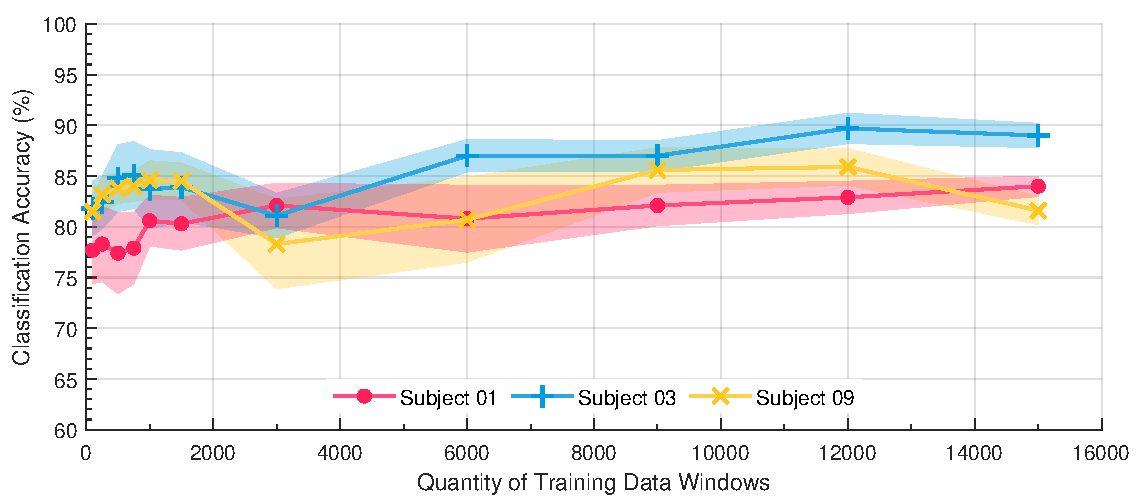
\includegraphics[width=0.95\textwidth]{content/5-Personalisation/ch5_frozen_lstm_layer_accuracy.pdf}
    \caption[Retraining a pre-trained LSTM model]{Retraining a pre-trained LSTM model - frozen LSTM layer}
    \label{fig:ch5_freezing_LSTM_layer}
\end{figure}

%-------------------------------------------------------------------------------
\section{Discussion}
\label{sec:personalisation-discussion}
What were we trying to achieve and have we achieved it?

Any interesting observations?

Bias the data set towards the target data, using the general population to supplement the limited environments experienced by the subject. Similar to Balanced Batch Learning \cite{Cruciani2020}

Reduced transition data from data set, previous work indicated these were a large source in inaccuracy.

Interesting how performance degrades at different increasing amounts of data. Suspicion is that this is because of the introduction of new environments of data. Limited control on data collection demonstrates problems with real world data. Encountering a new environment or mislabelling of data can result in degraded performance. Would be interesting to investigate how introduction of new environments affect performance but a new/different dataset collected in a controlled manner would be required for this

Do any of the methods show promise?

Identify requirements for implementing these methods (data, computation)

What are the limitations of this study/methods?

Areas for further work/improvements?

%-------------------------------------------------------------------------------
\section{Conclusions}
\label{sec:personalisation-conclusions}
What were the research aims?

Have we met the research aims/outcomes of this work?

What are we going to do next? Apply methods to amputee data and determine if they are applicable